\RequirePackage[l2tabu, orthodox]{nag}

%\documentclass[]{article}
\documentclass[11pt]{scrartcl}
\usepackage[usename, dvipsnames]{xcolor}
\usepackage[pdfencoding=auto]{hyperref}
\usepackage[msc-links]{amsrefs}
\usepackage{cleveref} % use \cref{}, automatically deduces theorem, proposition, etc
\usepackage[mathletters]{ucs}
\usepackage[utf8]{inputenc}
\usepackage[T1]{fontenc}
\usepackage{datetime}

\usepackage{array}
\usepackage{mathtools}
\usepackage{amsmath, amsthm, amssymb, amsfonts, amsxtra, amscd, thmtools}
\let\proof\relax
\let\endproof\relax

% Boxes around theorem environments.
\usepackage[many]{tcolorbox}

\usepackage{color}
%\usepackage{unicode-math}
\usepackage{newunicodechar}
\newunicodechar{ε}{\varepsilon}
\newunicodechar{δ}{\delta}
\newunicodechar{µ}{\mu}
\newunicodechar{→}{\to}
\newunicodechar{≤}{\leq}
\newunicodechar{∈}{\in}
\newunicodechar{⊆}{\subseteq}
\newunicodechar{Λ}{\Lambda}
\newunicodechar{∞}{\infty}
\newunicodechar{×}{\times}
\everymath{\displaystyle}



\usepackage{microtype}
\usepackage[pdfencoding=auto]{hyperref}
\usepackage{bookmark}
\usepackage{booktabs}
\usepackage{todonotes}
\usepackage[msc-links]{amsrefs}
\usepackage{cleveref} % use \cref{}, automatically deduces theorem, proposition, etc
\usepackage{csquotes}
\usepackage{longtable}
\usepackage{tabularx}
\usepackage{bbm}
% Creating multiple types of index
\usepackage{imakeidx}

% Remove indentation for new paragraphs
\usepackage{parskip}
% But leave space before amsthm environments
\makeatletter
\def\thm@space@setup{%
  \thm@preskip=2em
  \thm@postskip=2em
}
\makeatother


\usepackage{stmaryrd}
\usepackage{adjustbox}
\usepackage{centernot}
% \centernot\whatever


% Better indicator function
\usepackage{bbm}
\newcommand{\indic}[1]{\mathbbm{1} \left[ {#1} \right] }

% Highlight quote
\usepackage{environ}
\definecolor{camel}{rgb}{0.76, 0.6, 0.42}
\definecolor{babyblue}{rgb}{0.54, 0.81, 0.94}
\definecolor{block-gray}{gray}{0.85}
\NewEnviron{myblock}
{\colorbox{block-gray}{%
\parbox{\dimexpr\linewidth-2\fboxsep\relax}{%
\small\addtolength{\leftskip}{10mm}
\addtolength{\rightskip}{10mm}
\BODY}}
}
\renewcommand{\quote}{\myblock}
\renewcommand{\endquote}{\endmyblock}

% Nice math font that journals use
%\usepackage[lite]{mtpro2}
%\usepackage{mathrsfs}
%\usepackage{mathptmx}
\usepackage{lmodern}
%\usepackage[sc]{mathpazo}

% Theorem Styles
\usepackage[framemethod=tikz]{mdframed}

\theoremstyle{definition}
\newtheorem{exercise}{Exercise}[section]
\newtheorem{solution}{Solution}

% Theorem Style
\newtheoremstyle{theorem}% name
  {0em}%         Space above, empty = `usual value'
  {1em}%         Space below
  {\normalfont}% Body font
  {\parindent}%         Indent amount (empty = no indent, \parindent = para indent)
  {\bfseries}% Thm head font
  {.}%        Punctuation after thm head
  {\newline}% Space after thm head: \newline = linebreak
  {\thmname{#1}\thmnumber{ #2}\thmnote{\itshape{(#3)}}}%
\theoremstyle{theorem}
\tcolorboxenvironment{theorem}{
  boxrule=0pt,
  boxsep=0pt,
  breakable,
  enhanced jigsaw,
  fonttitle={\large\bfseries},
  opacityback=0.8,
  colframe=cyan,
  borderline west={4pt}{0pt}{orange},
  attach title to upper={}
}
\newtheorem{theorem}{Theorem}[section]

% Proposition Style
\tcolorboxenvironment{proposition}{
  boxrule=1pt,
  boxsep=0pt,
  breakable,
  enhanced jigsaw,
  opacityback=0.0,
  colframe=cyan
}
\newtheorem{proposition}[theorem]{Proposition}
\tcolorboxenvironment{lemma}{
  boxrule=1pt,
  boxsep=0pt,
  breakable,
  enhanced jigsaw,
  opacityback=0.2,
  colframe=cyan
}
\newtheorem{lemma}[theorem]{Lemma}
% Claim
\tcolorboxenvironment{claim}{
  boxrule=1pt,
  boxsep=0pt,
  breakable,
  enhanced jigsaw,
  opacityback=0.2,
  colframe=cyan
}
\newtheorem{claim}[theorem]{Claim}


% Corollary
\tcolorboxenvironment{corollary}{
  colback=cyan,
  boxrule=1pt,
  boxsep=0pt,
  breakable,
  enhanced jigsaw,
  opacityback=0.1,
  colframe=cyan
}
\newtheorem{corollary}[theorem]{Corollary}

% Proof Style
\newtheoremstyle{proof}% name
  {0em}%         Space above, empty = `usual value'
  {2em}%         Space below
  {\normalfont}% Body font
  {\parindent}%         Indent amount (empty = no indent, \parindent = para indent)
  {\itshape}% Thm head font
  {.}%        Punctuation after thm head
  {\newline}% Space after thm head: \newline = linebreak
  {\thmname{#1} \thmnote{\itshape{(#3)}}}%         Thm head spec
\theoremstyle{proof}
\tcolorboxenvironment{proof}{
  colback=camel,
  opacityfill=0.25,
  boxrule=1pt,
  boxsep=0pt,
  breakable,
  enhanced jigsaw
}
\newtheorem*{pf}{Proof}
\newenvironment{proof}
{\pushQED{$\qed$}\pf}
{\par\popQED\endpf}

% Definition Style
\newtheoremstyle{definition}% name
  {0em}%         Space above, empty = `usual value'
  {2em}%         Space below
  {\normalfont}% Body font
  {\parindent}%         Indent amount (empty = no indent, \parindent = para indent)
  {\bfseries}% Thm head font
  {.}%        Punctuation after thm head
  {\newline}% Space after thm head: \newline = linebreak
  {}%         Thm head spec
\theoremstyle{definition}
\tcolorboxenvironment{definition}{
  colback=babyblue,
  boxrule=0pt,
  boxsep=0pt,
  opacityfill=0.45,
  breakable,
  enhanced jigsaw,
  borderline west={4pt}{0pt}{blue},
  colbacktitle={babyblue},
  coltitle={black},
  fonttitle={\large\bfseries},
  attach title to upper={},
}
\newtheorem{definition}{Definition}[theorem]

% Break Environment
\makeatletter
\newtheoremstyle{break}% name
  {}%         Space above, empty = `usual value'
  {2em}%         Space below
  {
    \addtolength{\@totalleftmargin}{2.5em}
    \addtolength{\linewidth}{-2.5em}
    \parshape 1 2.5em \linewidth
  }% Body font
  {}%         Indent amount (empty = no indent, \parindent = para indent)
  {\bfseries}% Thm head font
  {.}%        Punctuation after thm head
  {\newline}% Space after thm head: \newline = linebreak
  {}%         Thm head spec
\makeatother

\theoremstyle{break}
\newtheorem{example}{Example}[section]

% Problem Style
\newtheoremstyle{problem} % name
  {0em}                   % Space above, empty = `usual value'
  {2em}                   % Space below
  {\normalfont}           % Body font
  {\parindent}            % Indent amount (empty = no indent, \parindent = para indent)
  {\itshape}              % Thm head font
  {}                      % Punctuation after thm head
  {\newline}              % Space after thm head: \newline = linebreak
  {\thmnote{\itshape{(#3)}}}     % Thm head spec
\theoremstyle{problem}
\tcolorboxenvironment{problem}{
  boxrule=1pt,
  boxsep=0pt,
  breakable,
  enhanced jigsaw,
  opacityback=0.0,
  colframe=cyan
}
\newtheorem{problem}{Problem}


%Pagination stuff.
\setlength{\topmargin}{-.3 in}
\setlength{\oddsidemargin}{0in}
\setlength{\evensidemargin}{0in}
\setlength{\textheight}{9.in}
\setlength{\textwidth}{6.5in}
% \pagestyle{empty} %removes page numbers.

% Inkscape figures from Vim
\usepackage{import}
\usepackage{pdfpages}
\usepackage{transparent}

\newcommand{\incfig}[1]{%
    \def\svgwidth{\columnwidth}
    \import{./figures/}{#1.pdf_tex}
}
%\pdfsuppresswarningpagegroup=1

% Pandoc-specific fixes
\providecommand{\tightlist}{%
  \setlength{\itemsep}{0pt}\setlength{\parskip}{0pt}}

% Tikz and Graphics
\usepackage{amscd}
\usepackage{tikz}
\usetikzlibrary{arrows, arrows.meta, cd, fadings, patterns, calc, decorations.markings, matrix, positioning}
\tikzfading[name=fade out, inner color=transparent!0, outer color=transparent!100]
\usepackage{pgfplots}
\pgfplotsset{compat=1.16}
\usepackage[inline]{asymptote}
\usepackage{tikz-layers}

%\usepackage{nath}
%\delimgrowth=1
\DeclarePairedDelimiter\qty{(}{)}

% Major Macros
\usepackage{graphicx}
\usepackage{float}
\DeclareFontFamily{U}{mathx}{\hyphenchar\font45}
\DeclareFontShape{U}{mathx}{m}{n}{
      <5> <6> <7> <8> <9> <10>
      <10.95> <12> <14.4> <17.28> <20.74> <24.88>
      mathx10
      }{}
\DeclareSymbolFont{mathx}{U}{mathx}{m}{n}
\DeclareMathSymbol{\bigtimes}{1}{mathx}{"91}

% Wide tikz equations
\newsavebox{\wideeqbox}
\newenvironment{wideeq}
  {\begin{displaymath}\begin{lrbox}{\wideeqbox}$\displaystyle}
  {$\end{lrbox}\makebox[0pt]{\usebox{\wideeqbox}}\end{displaymath}}



% Fancy chapter headers and footers
\usepackage{fancyhdr}

\pagestyle{fancy}
\fancyhf{}
\fancyhead[LE,RO]{\title}
\fancyhead[RE,LO]{\rightmark}
\fancyfoot[CE,CO]{\leftmark}
\fancyfoot[LE,RO]{\thepage}

\renewcommand{\headrulewidth}{2pt}
\renewcommand{\footrulewidth}{1pt}

% List of Theorems Attempt
\usepackage{etoolbox}
\makeatletter
\patchcmd\thmtlo@chaptervspacehack
  {\addtocontents{loe}{\protect\addvspace{10\p@}}}
  {\addtocontents{loe}{\protect\thmlopatch@endchapter\protect\thmlopatch@chapter{\thechapter}}}
  {}{}
\AtEndDocument{\addtocontents{loe}{\protect\thmlopatch@endchapter}}
\long\def\thmlopatch@chapter#1#2\thmlopatch@endchapter{%
  \setbox\z@=\vbox{#2}%
  \ifdim\ht\z@>\z@
    \hbox{\bfseries\chaptername\ #1}\nobreak
    #2
    \addvspace{10\p@}
  \fi
}
\def\thmlopatch@endchapter{}

\makeatother
\renewcommand{\thmtformatoptarg}[1]{ -- #1}
%\renewcommand{\listtheoremname}{List of definitions}

\newcommand{\ext}{\operatorname{Ext}}
\newcommand{\Ext}{\operatorname{Ext}}
\def\Endo{\operatorname{End}}
\def\Ind{\operatorname{Ind}}
\def\ind{\operatorname{Ind}}
\def\coind{\operatorname{Coind}}
\def\Res{\operatorname{Res}}
\def\Hol{\operatorname{Hol}}
\def\res{\operatorname{Res}}
\def\endo{\operatorname{End}}
\def\ind{\operatorname{Ind}}
\renewcommand{\AA}[0]{{\mathbb{A}}}
\DeclareMathOperator{\Exists}{\exists}
\DeclareMathOperator{\Forall}{\forall}
\newcommand{\Af}[0]{{\mathbb{A}}}
\newcommand{\CC}[0]{{\mathbb{C}}}
\newcommand{\CP}[0]{{\mathbb{CP}}}
\newcommand{\DD}[0]{{\mathbb{D}}}
\newcommand{\FF}[0]{{\mathbb{F}}}
\newcommand{\GF}[0]{{\mathbb{GF}}}
\newcommand{\GG}[0]{{\mathbb{G}}}
\newcommand{\HH}[0]{{\mathbb{H}}}
\newcommand{\HP}[0]{{\mathbb{HP}}}
\newcommand{\KK}[0]{{\mathbb{K}}}
\newcommand{\kk}[0]{{\Bbbk}}
\newcommand{\bbm}[0]{{\mathbb{M}}}
\newcommand{\NN}[0]{{\mathbb{N}}}
\newcommand{\OP}[0]{{\mathbb{OP}}}
\newcommand{\PP}[0]{{\mathbb{P}}}
\newcommand{\QQ}[0]{{\mathbb{Q}}}
\newcommand{\RP}[0]{{\mathbb{RP}}}
\newcommand{\RR}[0]{{\mathbb{R}}}
\newcommand{\SpSp}[0]{{\mathbb{S}}}
\renewcommand{\SS}[0]{{\mathbb{S}}}
\newcommand{\TT}[0]{{\mathbb{T}}}
\newcommand{\ZZ}[0]{{\mathbb{Z}}}
\newcommand{\ZnZ}[0]{\mathbb{Z}/n\mathbb{Z}}
\newcommand{\ZpZ}[0]{\mathbb{Z}/p\mathbb{Z}}
\newcommand{\Qp}[0]{\mathbb{Q}_{(p)}}
\newcommand{\Zp}[0]{\mathbb{Z}_{(p)}}
\newcommand{\Arg}[0]{\mathrm{Arg}}
\newcommand{\PGL}[0]{\mathrm{PGL}}
\newcommand{\GL}[0]{\mathrm{GL}}
\newcommand{\Gl}[0]{\mathrm{GL}}
\newcommand{\gl}[0]{\mathrm{GL}}
\newcommand{\mat}[0]{\mathrm{Mat}}
\newcommand{\Mat}[0]{\mathrm{Mat}}
\newcommand{\Rat}[0]{\mathrm{Rat}}
\newcommand{\Perv}[0]{\mathrm{Perv}}
\newcommand{\Gal}[0]{\mathrm{Gal}}
\newcommand{\Hilb}[0]{\mathrm{Hilb}}
\newcommand{\Quot}[0]{\mathrm{Quot}}
\newcommand{\Art}[0]{\mathrm{Art}}
\newcommand{\red}[0]{\mathrm{red}}
\newcommand{\alg}[0]{\mathrm{alg}}
\newcommand{\Pic}[0]{{\mathrm{Pic}~}}
\newcommand{\lcm}[0]{\mathrm{lcm}}
\newcommand{\maps}[0]{\mathrm{Maps}}
\newcommand{\maxspec}[0]{{\mathrm{maxSpec}~}}
\newcommand{\Tr}[0]{\mathrm{Tr}}
\newcommand{\adj}[0]{\mathrm{adj}}
\newcommand{\ad}[0]{\mathrm{ad}~}
\newcommand{\ann}[0]{\mathrm{Ann}}
\newcommand{\Ann}[0]{\mathrm{Ann}}
\newcommand{\arcsec}[0]{\mathrm{arcsec}}
\newcommand{\ch}[0]{\mathrm{char}~}
\newcommand{\Sp}[0]{{\mathrm{Sp}}}
\newcommand{\syl}[0]{{\mathrm{Syl}}}
\newcommand{\txand}[0]{{\text{ and }}}
\newcommand{\codim}[0]{\mathrm{codim}}
\newcommand{\txor}[0]{{\text{ or }}}
\newcommand{\txt}[1]{{\text{ {#1} }}}
\newcommand{\Gr}[0]{{\text{Gr}}}
\newcommand{\Aut}[0]{{\mathrm{Aut}}}
\newcommand{\aut}[0]{\mathrm{Aut}}
\newcommand{\Inn}[0]{{\mathrm{Inn}}}
\newcommand{\Out}[0]{{\mathrm{Out}}}
\newcommand{\mltext}[1]{\left\{\begin{array}{c}#1\end{array}\right\}}
\newcommand{\Fun}[0]{{\text{Fun}}}
\newcommand{\SL}[0]{{\text{SL}}}
\newcommand{\PSL}[0]{{\text{PSL}}}
\newcommand{\SO}[0]{{\text{SO}}}
\newcommand{\SU}[0]{{\text{SU}}}
\newcommand{\SP}[0]{{\text{SP}}}
\newcommand{\per}[0]{{\text{Per}}}
\newcommand{\loc}[0]{{\text{loc}}}
\newcommand{\Top}[0]{{\text{Top}}}
\newcommand{\Sch}[0]{{\text{Sch}}}
\newcommand{\sch}[0]{{\text{Sch}}}
\newcommand{\Set}[0]{{\text{Set}}}
\newcommand{\Sets}[0]{{\text{Set}}}
\newcommand{\Grp}[0]{{\text{Grp}}}
\newcommand{\Groups}[0]{{\text{Groups}}}
\newcommand{\Homeo}[0]{{\text{Homeo}}}
\newcommand{\Diffeo}[0]{{\text{Diffeo}}}
\newcommand{\MCG}[0]{{\text{MCG}}}
\newcommand{\set}[0]{{\text{Set}}}
\newcommand{\Tor}[0]{\text{Tor}}
\newcommand{\sets}[0]{{\text{Set}}}
\newcommand{\Sm}[0]{{\text{Sm}_k}}
\newcommand{\orr}[0]{{\text{ or }}}
\newcommand{\annd}[0]{{\text{ and }}}
\newcommand{\bung}[0]{\text{Bun}_G}
\newcommand{\const}[0]{{\text{const.}}}
\newcommand{\disc}[0]{{\text{disc}}}
\newcommand{\op}[0]{^\text{op}}
\newcommand{\id}[0]{\text{id}}
\newcommand{\im}[1]{\mathrm{im}({#1})}
\newcommand{\pt}[0]{{\{\text{pt}\}}}
\newcommand{\sep}[0]{^\text{sep}}
% \newcommand{\st}[0]{~{\text{s.t.}}~}
\newcommand{\tors}[0]{{\text{tors}}}
\newcommand{\tor}[0]{\text{Tor}}
\newcommand{\height}[0]{\text{ht}}
\newcommand{\cpt}[0]{\text{compact}}
\newcommand{\abs}[1]{{\left\lvert {#1} \right\rvert}}
\newcommand{\stack}[1]{\mathclap{\substack{ #1 }}} 
\newcommand{\qtext}[1]{{\quad \text{#1} \quad}}
\newcommand{\qst}[0]{{\quad \text{such that} \quad}}
\newcommand{\actsonl}[0]{\curvearrowleft}
\newcommand{\actson}[0]{\curvearrowright}
\newcommand{\bd}[0]{{\del}}
\newcommand{\bigast}[0]{{\mathop{\Large \ast}}}
\newcommand{\coker}[0]{\operatorname{coker}}
\newcommand{\cok}[0]{\operatorname{coker}}
\newcommand{\conjugate}[1]{{\overline{{#1}}}}
\newcommand{\converges}[1]{\overset{#1}}
\newcommand{\correspond}[1]{\theset{\substack{#1}}}
\newcommand{\cross}[0]{\times}
\newcommand{\by}[0]{\times}
\newcommand{\dash}[0]{{\hbox{-}}}
\newcommand{\dd}[2]{{\frac{\partial #1}{\partial #2}\,}}
\newcommand{\definedas}[0]{\coloneqq}
\newcommand{\da}[0]{\coloneqq}
\newcommand{\del}[0]{{\partial}}
\newcommand{\directlim}[0]{\varinjlim}
\newcommand{\disjoint}[0]{{\coprod}}
\newcommand{\divides}[0]{{~\Bigm|~}}
\newcommand{\dual}[0]{^\vee}
\newcommand{\sm}[0]{\setminus}
\newcommand{\smz}[0]{\setminus\theset{0}}
\newcommand{\eps}[0]{\varepsilon}
\newcommand{\equalsbecause}[1] {\stackrel{\mathclap{\scriptscriptstyle{#1}}}{=}}
\newcommand{\floor}[1]{{\left\lfloor #1 \right\rfloor}}
\DeclarePairedDelimiter{\ceil}{\lceil}{\rceil}
\newcommand{\from}[0]{\leftarrow}
\newcommand{\tofrom}[0]{\leftrightarrows}
\newcommand{\up}[0]{\uparrow}
\newcommand{\generators}[1]{\left\langle{#1}\right\rangle}
\newcommand{\gs}[1]{\left\langle{#1}\right\rangle}
\newcommand{\homotopic}[0]{\simeq}
\newcommand{\injectivelim}[0]{\varinjlim}
\newcommand{\injects}[0]{\hookrightarrow}
\newcommand{\inner}[2]{{\left\langle {#1},~{#2} \right\rangle}}
\newcommand{\union}[0]{\cup}
\newcommand{\Union}[0]{\bigcup}
\newcommand{\intersect}[0]{\cap}
\newcommand{\Intersect}[0]{\bigcap}
\newcommand{\into}[0]{\to}
\newcommand{\inverselim}[0]{\varprojlim}
\newcommand{\inv}[0]{^{-1}}
\newcommand{\mfa}[0]{{\mathfrak{a}}}
\newcommand{\mfb}[0]{{\mathfrak{b}}}
\newcommand{\mfc}[0]{{\mathfrak{c}}}
\newcommand{\mff}[0]{{\mathfrak{f}}}
\newcommand{\mfi}[0]{{\mathfrak{I}}}
\newcommand{\mfm}[0]{{\mathfrak{m}}}
\newcommand{\mfn}[0]{{\mathfrak{n}}}
\newcommand{\mfp}[0]{{\mathfrak{p}}}
\newcommand{\mfq}[0]{{\mathfrak{q}}}
\newcommand{\mfr}[0]{{\mathfrak{r}}}
\newcommand{\lieb}[0]{{\mathfrak{b}}}
\newcommand{\liegl}[0]{{\mathfrak{gl}}}
\newcommand{\lieg}[0]{{\mathfrak{g}}}
\newcommand{\lieh}[0]{{\mathfrak{h}}}
\newcommand{\lien}[0]{{\mathfrak{n}}}
\newcommand{\liesl}[0]{{\mathfrak{sl}}}
\newcommand{\lieso}[0]{{\mathfrak{so}}}
\newcommand{\liesp}[0]{{\mathfrak{sp}}}
\newcommand{\lieu}[0]{{\mathfrak{u}}}
\newcommand{\nilrad}[0]{{\mathfrak{N}}}
\newcommand{\jacobsonrad}[0]{{\mathfrak{J}}}
\newcommand{\mm}[0]{{\mathfrak{m}}}
\newcommand{\pr}[0]{{\mathfrak{p}}}
\newcommand{\mapsvia}[1]{\xrightarrow{#1}}
\newcommand{\kx}[1]{k[x_1, \cdots, x_{#1}]}
\newcommand{\MM}[0]{{\mathcal{M}}}
\newcommand{\OO}[0]{{\mathcal{O}}}
\newcommand{\imaginarypart}[1]{{\mathcal{Im}({#1})}}
\newcommand{\mca}[0]{{\mathcal{A}}}
\newcommand{\mcb}[0]{{\mathcal{B}}}
\newcommand{\mcc}[0]{{\mathcal{C}}}
\newcommand{\mcd}[0]{{\mathcal{D}}}
\newcommand{\mce}[0]{{\mathcal{E}}}
\newcommand{\mcf}[0]{{\mathcal{F}}}
\newcommand{\mcg}[0]{{\mathcal{G}}}
\newcommand{\mch}[0]{{\mathcal{H}}}
\newcommand{\mci}[0]{{\mathcal{I}}}
\newcommand{\mcj}[0]{{\mathcal{J}}}
\newcommand{\mck}[0]{{\mathcal{K}}}
\newcommand{\mcl}[0]{{\mathcal{L}}}
\newcommand{\mcm}[0]{{\mathcal{M}}}
\newcommand{\mcp}[0]{{\mathcal{P}}}
\newcommand{\mcs}[0]{{\mathcal{S}}}
\newcommand{\mct}[0]{{\mathcal{T}}}
\newcommand{\mcu}[0]{{\mathcal{U}}}
\newcommand{\mcv}[0]{{\mathcal{V}}}
\newcommand{\mcx}[0]{{\mathcal{X}}}
\newcommand{\mcz}[0]{{\mathcal{Z}}}
\newcommand{\cl}[0]{\mathrm{cl}}
\newcommand{\trdeg}[0]{\mathrm{trdeg}}
\newcommand{\dist}[0]{\mathrm{dist}}
\newcommand{\Dist}[0]{\mathrm{Dist}}
\newcommand{\crit}[0]{\mathrm{crit}}
\newcommand{\diam}[0]{{\mathrm{diam}}}
\newcommand{\gal}[0]{\mathrm{Gal}}
\newcommand{\diff}[0]{\mathrm{Diff}}
\newcommand{\diag}[0]{\mathrm{diag}}
\newcommand{\soc}[0]{\mathrm{Soc}\,}
\newcommand{\hd}[0]{\mathrm{Head}\,}
\newcommand{\grad}[0]{\mathrm{grad}~}
\newcommand{\hilb}[0]{\mathrm{Hilb}}
\newcommand{\minpoly}[0]{{\mathrm{minpoly}}}
\newcommand{\Hom}[0]{{\mathrm{Hom}}}
\newcommand{\Map}[0]{{\mathrm{Map}}}
\newcommand{\multinomial}[1]{\left(\!\!{#1}\!\!\right)}
\newcommand{\nil}[0]{{\mathrm{nil}}}
\newcommand{\normalneq}{\mathrel{\reflectbox{$\trianglerightneq$}}}
\newcommand{\normal}[0]{{~\trianglelefteq~}}
\newcommand{\norm}[1]{{\left\lVert {#1} \right\rVert}}
\newcommand{\pnorm}[2]{{\left\lVert {#1} \right\rVert}_{#2}}
\newcommand{\notdivides}[0]{\nmid}
\newcommand{\onto}[0]{\twoheadhthtarrow}
\newcommand{\ord}[0]{{\mathrm{Ord}}}
\newcommand{\pic}[0]{{\mathrm{Pic}~}}
\newcommand{\projectivelim}[0]{\varprojlim}
\newcommand{\rad}[0]{{\mathrm{rad}~}}
\newcommand{\ralg}[0]{\mathrm{R-alg}}
\newcommand{\kalg}[0]{k\dash\mathrm{alg}}
\newcommand{\rank}[0]{\operatorname{rank}}
\newcommand{\realpart}[1]{{\mathcal{Re}({#1})}}
\newcommand{\Log}[0]{\mathrm{Log}}
\newcommand{\reg}[0]{\mathrm{Reg}}
\newcommand{\restrictionof}[2]{{\left.{#1}\right|_{#2}}}
\newcommand{\ro}[2]{{\left.{#1}\right|_{#2}}}
\newcommand{\rk}[0]{{\mathrm{rank}}}
\newcommand{\evalfrom}[0]{\Big|}
\newcommand{\rmod}[0]{{R\dash\mathrm{mod}}}
\newcommand{\Mod}[0]{{\mathrm{Mod}}}
\newcommand{\rotate}[2]{{\style{display: inline-block; transform: rotate(#1deg)}{#2}}}
\newcommand{\selfmap}[0]{{\circlearrowleft}}
\newcommand{\semidirect}[0]{\rtimes}
\newcommand{\sgn}[0]{\mathrm{sgn}}
\newcommand{\sign}[0]{\mathrm{sign}}
\newcommand{\spanof}[0]{{\mathrm{span}}}
\newcommand{\spec}[0]{\mathrm{Spec}\,}
\newcommand{\mspec}[0]{\mathrm{mSpec}~}
\newcommand{\stab}[0]{{\mathrm{Stab}}}
\newcommand{\stirlingfirst}[2]{\genfrac{[}{]}{0pt}{}{#1}{#2}}
\newcommand{\stirling}[2]{\genfrac\{\}{0pt}{}{#1}{#2}}
\newcommand{\strike}[1]{{\enclose{horizontalstrike}{#1}}}
\newcommand{\suchthat}[0]{{~\mathrel{\Big|}~}}
\newcommand{\st}[0]{{~\mathrel{\Big|}~}}
\newcommand{\supp}[0]{{\mathrm{supp}}}
\newcommand{\surjects}[0]{\twoheadrightarrow}
\newcommand{\sym}[0]{\mathrm{Sym}}
\newcommand{\tensor}[0]{\otimes}
\newcommand{\connectsum}[0]{\mathop{\Large \#}}
\newcommand{\theset}[1]{\left\{{#1}\right\}}
\newcommand{\ts}[1]{\left\{{#1}\right\}}
\newcommand{\gens}[1]{\left\langle{#1}\right\rangle}
\newcommand{\thevector}[1]{{\left[ {#1} \right]}}
\newcommand{\tv}[1]{{\left[ {#1} \right]}}
\newcommand{\too}[1]{{\xrightarrow{#1}}}
\newcommand{\transverse}[0]{\pitchfork}
\newcommand{\trianglerightneq}{\mathrel{\ooalign{\raisebox{-0.5ex}{\reflectbox{\rotatebox{90}{$\nshortmid$}}}\cr$\triangleright$\cr}\mkern-3mu}}
\newcommand{\tr}[0]{\mathrm{Tr}}
\newcommand{\uniformlyconverges}[0]{\rightrightarrows}
\newcommand{\covers}[0]{\rightrightarrows}
\newcommand{\units}[0]{^{\times}}
\newcommand{\nonzero}[0]{^{\bullet}}
\newcommand{\wait}[0]{{\,\cdot\,}}
\newcommand{\wt}[0]{{\mathrm{wt}}}
\renewcommand{\bar}[1]{\mkern 1.5mu\overline{\mkern-1.5mu#1\mkern-1.5mu}\mkern 1.5mu}
\renewcommand{\div}[0]{\mathrm{Div}}
\newcommand{\Div}[0]{\mathrm{Div}}
\renewcommand{\hat}[1]{\widehat{#1}}
\renewcommand{\mid}[0]{\mathrel{\Big|}}
\renewcommand{\qed}[0]{\hfill\blacksquare}
\renewcommand{\too}[0]{\longrightarrow}
\renewcommand{\vector}[1]{\mathbf{#1}}
\let\oldexp\exp
\renewcommand{\exp}[1]{\oldexp\qty{#1}}
\let\oldperp\perp
\renewcommand{\perp}[0]{^\oldperp}
\newcommand*\dif{\mathop{}\!\mathrm{d}}
\newcommand{\ddt}{\tfrac{\dif}{\dif t}}
\newcommand{\ddx}{\tfrac{\dif}{\dif x}}

\DeclareMathOperator{\righttriplearrows} {{\; \tikz{ \foreach \y in {0, 0.1, 0.2} { \draw [-stealth] (0, \y) -- +(0.5, 0);}} \; }}



\addbibresource{EtaleCohomology.bib}

\let\Begin\begin
\let\End\end
\newcommand\wrapenv[1]{#1}

\makeatletter
\def\ScaleWidthIfNeeded{%
 \ifdim\Gin@nat@width>\linewidth
    \linewidth
  \else
    \Gin@nat@width
  \fi
}
\def\ScaleHeightIfNeeded{%
  \ifdim\Gin@nat@height>0.9\textheight
    0.9\textheight
  \else
    \Gin@nat@width
  \fi
}
\makeatother

\setkeys{Gin}{width=\ScaleWidthIfNeeded,height=\ScaleHeightIfNeeded,keepaspectratio}%

\title{
\rule{\linewidth}{1pt} \\
\textbf{
    Étale Cohomology
  }
    \\ {\normalsize University of Georgia, Fall 2020} \\
  \rule{\linewidth}{2pt}
}
\titlehead{
    \begin{center}
  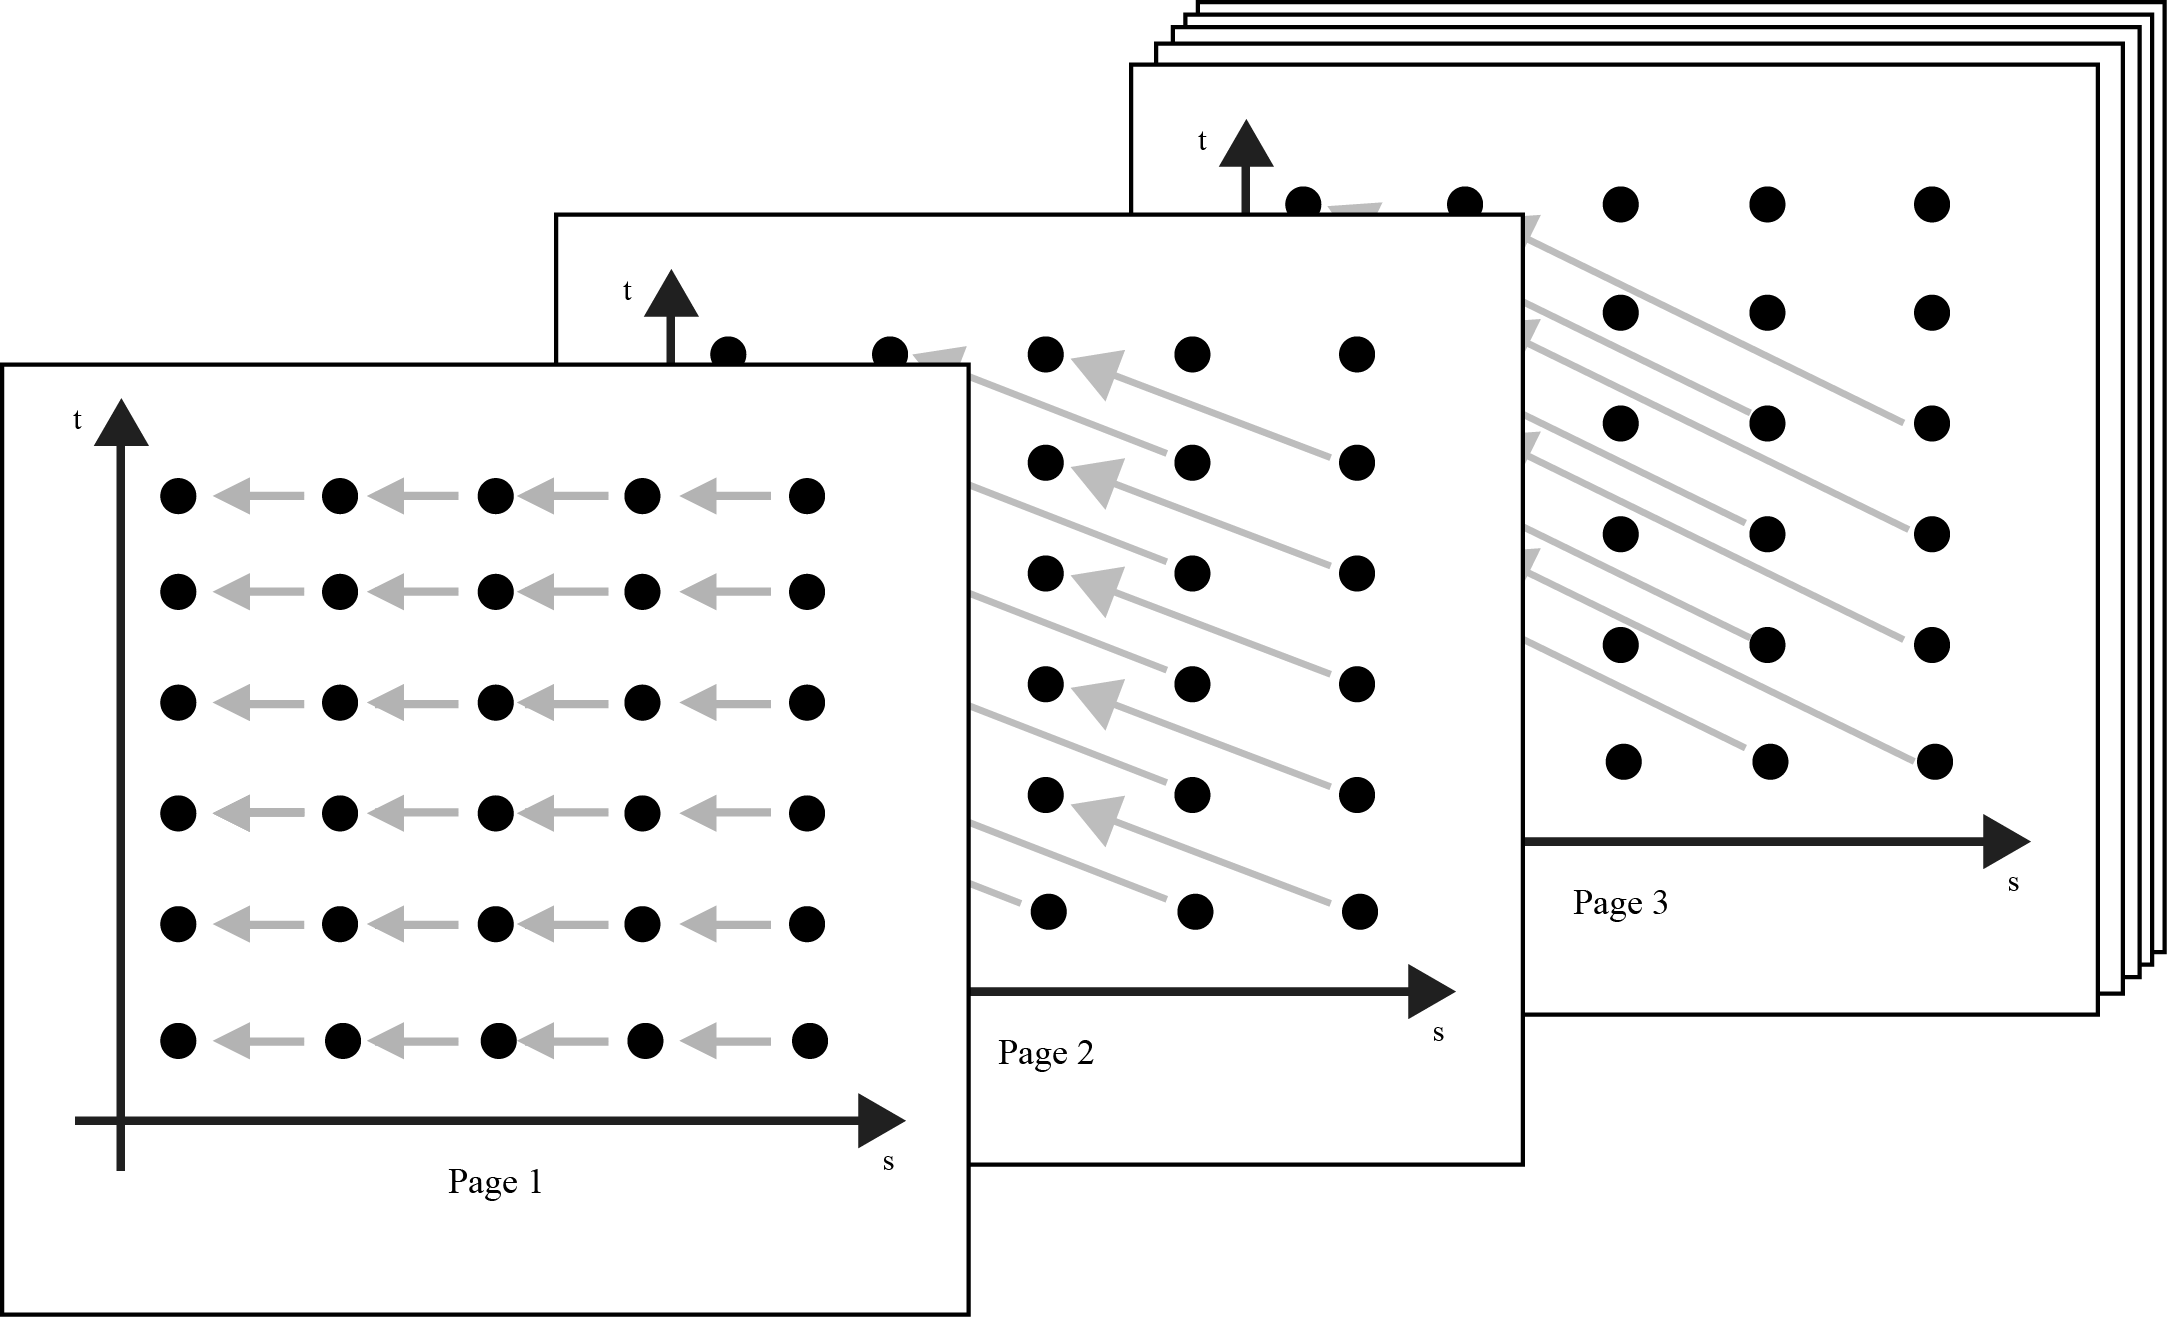
\includegraphics[width=\linewidth,height=0.45\textheight,keepaspectratio]{figures/cover.png}
  \end{center}
       \begin{minipage}{.35\linewidth}
    \begin{flushleft}
      \vspace{2em}
      {\fontsize{6pt}{2pt} \textit{Notes: These are notes live-tex'd
from a graduate course on Étale Cohomology taught by Daniel Litt at the
University of Georgia in Fall 2020. As such, any errors or inaccuracies
are almost certainly my own. } } \\
    \end{flushleft}
    \end{minipage}
    \hfill
    \begin{minipage}{.65\linewidth}
    \end{minipage}
  }







\begin{document}

\date{}
\author{D. Zack Garza}
\maketitle
\begin{flushleft}
\textit{D. Zack Garza} \\
\textit{University of Georgia} \\
  \textit{\href{mailto: dzackgarza@gmail.com}{dzackgarza@gmail.com}} \\
{\tiny \textit{Last updated:} 2020-12-26 }
\end{flushleft}


\newpage

% Note: addsec only in KomaScript
\addsec{Table of Contents}
\tableofcontents
\newpage

These are notes live-tex'd from a graduate course in Étale Cohomology
taught by Daniel Litt at the University of Georgia in Fall 2020. As
such, any errors or inaccuracies are almost certainly my own.

\medskip
\begin{flushright}
  D. Zack Garza, \today \\
  \currenttime
\end{flushright}

\hypertarget{lecture-1}{%
\section{Lecture 1}\label{lecture-1}}

\hypertarget{references}{%
\subsection{References}\label{references}}

\begin{itemize}
\tightlist
\item
  \url{https://www.daniellitt.com/tale-cohomology}
\item
  \autocite{milneLEC}, \autocite{milne_2017},
  \autocite{freitag_kiehl_2013}, \autocite{katz}
\end{itemize}

\hypertarget{intro}{%
\subsection{Intro}\label{intro}}

Prerequisites:

\begin{itemize}
\tightlist
\item
  Homological Algebra

  \begin{itemize}
  \tightlist
  \item
    Abelian Categories
  \item
    Derived Functors
  \item
    Spectral Sequences (just exposure!)
  \end{itemize}
\item
  Sheaf theory and sheaf cohomology
\item
  Schemes (Hartshorne II and III)
\end{itemize}

Outline/Goals:

\begin{itemize}
\tightlist
\item
  Basics of etale cohomology

  \begin{itemize}
  \tightlist
  \item
    Etale morphism
  \item
    Grothendieck topologies
  \item
    The etale topology
  \item
    Etale cohomology and the basis theorems
  \item
    Etale cohomology of curves
  \item
    Comparison theorems to singular cohomology
  \item
    Focused on the case where coefficients are a constructible sheaf.
  \end{itemize}
\item
  Prove the Weil Conjectures (more than one proof)

  \begin{itemize}
  \tightlist
  \item
    Proving the Riemann Hypothesis for varieties over finite fields
  \end{itemize}

  \begin{quote}
  One of the greatest pieces of 20th century mathematics!
  \end{quote}
\item
  Topics

  \begin{itemize}
  \tightlist
  \item
    Weil 2 (Strengthening of RH, used in practice)
  \item
    Formality of algebraic varieties (topological features unique to
    varieties)
  \item
    Other things (monodromy, refer to Katz' AWS notes)
  \end{itemize}
\end{itemize}

\hypertarget{what-is-etale-cohomology}{%
\subsection{What is Etale Cohomology?}\label{what-is-etale-cohomology}}

Suppose \(X/\CC\) is a quasiprojective variety: a finite type separated
integral \(\CC\dash\)scheme. If you take the complex points, it
naturally has the structure of a complex analytic space
\(X(\CC)^{\text{an}}\): you can give it the Euclidean topology, which is
much finer than the Zariski topology. For a nice topological space, we
can associate the singular cohomology \(H^i(X(\CC)^{\text{an}}, \ZZ)\),
which satisfies several nice properties:

\begin{itemize}
\tightlist
\item
  Finitely generated \(\ZZ\dash\)modules
\item
  Extra Hodge structure when tensored up to \(\CC\) (same as \(\CC\)
  coefficients)
\item
  Cycle classes (i.e.~associate to a subvariety a class in cohomology)
\end{itemize}

Goal of etale cohomology: do something similar for much more general
``nice'' schemes. Note that some of these properties are special to
complex varieties. (E.g. finitely generated: not true for a random
topological space.)

We'll associate \(X\) a ``nice scheme''
\(\rightsquigarrow H^i(X_{\text{et}}, \ZZ/\ell^n\ZZ)\). Take the inverse
limit over all \(n\) to obtain the \(\ell\dash\)adic cohomology
\(H^i(X_{\text{et}}, \ZZ_\ell)\). You can tensor with \(\QQ\) to get
something with \(\QQ_\ell\) coefficients. And as in singular cohomology,
you can a ``twisted coefficient system''.

\begin{example}[?]

What are some nice schemes?

\begin{itemize}
\tightlist
\item
  \(X = \spec \OO_k\), the ring of integers over a number field.
\item
  \(X\) a variety over an algebraically closed field

  \begin{itemize}
  \tightlist
  \item
    Typical, most analogous to taking a variety over \(\CC\).
  \end{itemize}
\item
  \(X\) a variety over a non-algebraically closed field
\end{itemize}

\end{example}

Some comparisons between the last two cases:

\begin{itemize}
\tightlist
\item
  For \(\CC\dash\) variety, \(H^i_{\text{sing}}\) will vanish above
  \(i=2d\).
\item
  Over a finite field, \(H^i\) will vanish for \(i>2d+1\) but generally
  not vanish for \(i=2d+1\).
\end{itemize}

In good situations, these are finitely generated
\(\ZZ/\ell^n\ZZ\dash\)modules, have Mayer-Vietoris and excision
sequences, spectral sequences, etc. Related invariants: for a scheme
with a geometric point \footnote{A \textbf{geometric point} is a map
  from \(\spec X\) to an algebraically closed field.}

\((X, \bar x) \rightsquigarrow \pi_1^{\text{étale}}(X, \bar x)\), which
is a profinite topological group, which is a profinite topological
group.

\begin{remark}

More invariants beyond the scope of this course:

\begin{itemize}
\tightlist
\item
  Higher homotopy groups
\item
  Homotopy type (equivalence class of spaces)
\end{itemize}

So we want homotopy-theoretic invariants for varieties.

\end{remark}

\begin{remark}

This cohomology theory is necessarily weird! The following theorem
explains why. The slogan: there is no cohomology theory with \(\QQ\)
coefficients.

\end{remark}

\begin{theorem}[Serre]

There does not exists a cohomology theory for schemes over
\(\bar{\FF}_q\) with the following properties:

\begin{enumerate}
\def\labelenumi{\arabic{enumi}.}
\tightlist
\item
  Functorial
\item
  Satisfies the Kunneth formula
\item
  For \(E\) an elliptic curve, \(H^1(E) = \QQ^2\).
\end{enumerate}

\end{theorem}

\begin{proof}

Take \(E\) to be a supersingular elliptic curve. Then
\(\endo(E) \tensor \QQ\) is a quaternion algebra, and use the fact that
there are no algebra morphisms \(R\to \mat_{2\times 2}(\QQ)\).

\end{proof}

\begin{exercise}

Functoriality and Kunneth implies that \(\endo(E)\actson E\) yields an
action on \(H^1(E)\), which is precisely an algebra morphism
\(\endo(E) \to \mat_{2\by 2}(\QQ)\), a contradiction.

The content here: the sum of two endomorphisms act via their sum on
\(H^1\).

\end{exercise}

\begin{exercise}

Prove the same thing for \(\QQ_p\) coefficients, where \(p\) divides the
characteristic of the ground field. Proof the same, just need to know
what quaternion algebras show up.

\end{exercise}

This forces using some funky type of coefficients.

\hypertarget{what-are-the-weil-conjectures}{%
\subsection{What are the Weil
Conjectures?}\label{what-are-the-weil-conjectures}}

Suppose \(X/\FF_q\) is a variety, then
\begin{align*}  
\zeta_X(t) = \exp{\sum_{n>0} { {\abs{X(\FF_{q^n})} \over n} t^n } }
.\end{align*}

\begin{remark}

\envlist

\begin{itemize}
\item
  \(\dd{}{t} \log \zeta_X(t)\) is an ordinary generating function for
  the number of rational points.
\item
  Slogan: locations of zeros and poles of a meromorphic function control
  the growth rate of the coefficients of the Taylor series of the
  logarithmic derivative.
\end{itemize}

\end{remark}

\begin{exercise}

Make this slogan precise for rational functions, i.e.~ratios of two
polynomials.

\end{exercise}

\begin{theorem}[The Weil Conjectures]

\envlist

\begin{enumerate}
\def\labelenumi{\arabic{enumi}.}
\item
  \(\zeta_x(t)\) is a rational function.
\item
  (Functional equation) For \(X\) smooth and proper
  \begin{align*}  
  \zeta_X(q^{-n} t\inv) = \pm q^{nE \over 2} t^E \zeta_X(t)
  .\end{align*}
\item
  (RH) All roots and poles of \(\zeta_X(t)\) have absolute value
  \(q^{i\over 2}\) with \(i\in \ZZ\), and these are equal to the \(i\)th
  Betti numbers if \(X\) lifts to characteristic zero.\footnote{Note
    that we'll generalize Betti numbers so this makes sense in general.}
\end{enumerate}

\end{theorem}

\begin{remark}

These are all theorems! The proofs:

\begin{enumerate}
\def\labelenumi{\arabic{enumi}.}
\item
  Dwork, using \(p\dash\)adic methods. Proof here will follow from the
  fact that \(H^i_{\text{étale} }\) are finite-dimensional. Related to
  the \textbf{Lefschetz Trace Formula}, and is how Grothendieck thought
  about it.
\item
  Grothendieck, follows from some version of Poincaré duality.
\item
  (and 4) Deligne.
\end{enumerate}

\end{remark}

\hypertarget{euler-product}{%
\subsubsection{Euler Product}\label{euler-product}}

Let \(\abs X\) denote the closed points of \(X\), then there is an Euler
product:
\begin{align*}  
\zeta_X(q^{-n} t\inv) = \pm q^{nE \over 2} t^E \zeta_X(t)
&= \prod_{x\in \abs{X}} \exp{t^{\deg (x)} + {t^{2\deg (x)} \over 2} + \cdots} \\
&= \prod_{x\in \abs X} \exp{-\log(1-t^{\deg(x)})} \\
&= \prod_{x\in \abs X} {1 \over 1 - t^{\deg(x)}}
.\end{align*}

\begin{exercise}

Check the first equality. If you have a point of \(\deg(x) = n\), how
many \(\FF_{q^n}\) points does this contribute? I.e., how many maps are
there \(\spec(\FF_{q^n}) \to \spec(\FF_{q^n})\) over \(\FF_q\)?

There are exactly \(n\): it's \(\gal(\FF_{q^n} / \FF_q)\). But then
division by \(n\) drops this contribution to one.

\end{exercise}

We can keep going by expanding and multiplying out the product:
\begin{align*}  
\prod_{x\in \abs X} {1 \over 1 - t^{\deg(x)}}
&= \prod_{x\in \abs X} (1 + t^{\deg(x)} + t^{2 \deg(x)}) \\
&= \sum_{n\geq 0} \qty{\text{\# of Galois-stable subset of $X(\bar \FF_{q^n})$ of size $n$}}t^n
.\end{align*}

Why? If you have a degree \(x\) point, it contributes a stable subset of
size \(x\): namely the \(\FF_{q^n}\) points of \(\FF_{q^n}\). Taking
Galois orbits like that correspond to multiplying this product. But
these are the points of some algebraic variety:
\begin{align*}  
\cdots 
= \sum_{n\geq 0} \abs{\sym^n(X)(\FF_q)} t^n
,\end{align*} where \(\sym^n(X) \da X^n/\Sigma_n\), the action of the
symmetric group. Why is that? A \(\bar \FF_q\) point of \(\sym^n(X)\) is
an unordered \(n\dash\)tuple of \(\bar \FF_q\) points without an
ordering, and asking them to be Galois stable is the same as saying that
they are an \(\FF_q\) point.

\begin{theorem}[First Weil Conjecture for Curves]

For \(X\) a smooth proper curve over \(\FF_q\), \(\zeta_X(t)\) is
rational.

\end{theorem}

\begin{proof}

\begin{claim}

There is a set map
\begin{align*}  
\sym^n X &\to \pic^n X \\
D &\mapsto \OO(D)
,\end{align*} where here the divisor is an \(n\dash\)tuple of points.

\end{claim}

What are the fibers over a line bundle \(\OO(D)\)? A linear system,
i.e.~the projectivization of global sections \(\PP \Gamma(X, \OO(D))\).
What is the expected dimension? To compute the dimension of the space of
line bundles on a curve, use Riemann-Roch:
\begin{align*}  
\dim \PP\Gamma(X, \OO(D)) = \deg(D) + 1 - g + \dim H^1(X, \OO(D)) - 1
.\end{align*} where the last \(-1\) comes from the fact that this is a
projective space.

\begin{claim}

If \(\deg(D) = 2g-2\), then \(H^1(X, \OO(D)) = 0\).

\end{claim}

This is because it's dual to \(H^0(X, \OO(K-D))\dual\), but this has
negative degree and a line bundle of negative degree can never have
sections.\footnote{You should check to make sure you know why this is
  true!} Thus the fibers are isomorphic to \(\PP^{n-g}\) for \(n>2g-2\).
Now make a reduction\footnote{Exercise: justify why the reduction is
  valid.} and without loss of generality, assume
\(X(\FF_q) \neq \emptyset\). In this case,
\(\pic^n(X) \cong \pic^{n+1}(X)\) for all \(n\), since you can take
\(\OO(P)\) for \(P\) a point, a degree 1 line bundle, and tensor with
it. It's an isomorphism because you can tensor with the dual bundle to
go back. Thus for all \(n>2g-2\),
\begin{align*}  
\abs{\sym^n(X)(\FF_q)} 
= \abs{\PP^{n-g}(\FF_q)} \cdot \abs{\pic^n(X)(\FF_q)}
= \abs{\PP^{n-g}(\FF_q)} \cdot \abs{\pic^0(X)(\FF_q)}
.\end{align*}

Thus \(\zeta_X(t)\) is a polynomial plus
\(\sum_{n>2g-2} \abs{\pic^n(X)(\FF_q)}\qty{1+q+q^2+\cdots+q^{n-g}}t^n\).

\begin{exercise}

Show that this is a rational function using the formula for a geometric
series.

\end{exercise}

\end{proof}

\begin{theorem}[Functional Equation]

The functional equation in the case of curves:
\begin{align*}  
\zeta_X(q^{-1} t^{-1} ) = \pm q^{2-2g \over 2} t^{2-2g} \zeta_X(t)
.\end{align*}

\end{theorem}

\begin{exercise}[Important]

Where it comes from in terms of \(\sym^n\): Serre duality.

\end{exercise}

We'll show the RH later.

\begin{theorem}[Dwork]

Suppose \(X/\FF_q\) is any variety, then \(\zeta_X(t)\) is rational
function.

\end{theorem}

This was roughly known to Weil, hinted at in original paper

\begin{proof}[Grothendieck]

Idea: take Frobenius (intentionally vague, arithmetic vs geometric vs
\ldots) \(F:X\to X\), then \(X(\FF_q)\) are the fixed points of \(F\)
acting on \(X_{\bar \FF_q}\), and the \(\FF_{q^n}\) points are the fixed
points of \(F^n\). Uses the Lefschetz fixed point formula, which will
say for \(\ell\neq \ch(\FF_q)\),\footnote{Here \(H^i_c\) is compactly
  supported cohomology, we'll define this later in the course.}

\begin{align*}  
\abs{X(\FF_{q^n})} = \sum_{i=0}^{2\dim(X)} (-1)^i \tr(F^n) H^i_c(X_{\FF_q}, \QQ_\ell)
.\end{align*}

\begin{lemma}

\begin{align*}  
\exp{\sum {\tr(F^n) \over n}t^n  }\quad\text{is rational}
.\end{align*}

\end{lemma}

This lemma implies the result, because if you plug the trace formula
into the zeta function, you'll get an alternating product
\(f \cdots {1\over g} \cdot h \cdot {1\over j} \cdots\) of functions of
the form in the lemma, which is still rational.

\end{proof}

\begin{proof}[Of Lemma]

It suffices to treat the case \(\dim(V) = 1\), because otherwise you can
just write this as a sum of powers of eigenvalues. Then you have a
scalar matrix, so you obtain
\begin{align*}  
\exp{ \sum {\alpha^n \over n} t^n} = \exp{ -\log(1 - \alpha t)} = {1 \over 1-\alpha t}
,\end{align*} which is rational.

\end{proof}

This proves rationality, contingent on

\begin{enumerate}
\def\labelenumi{\arabic{enumi}.}
\tightlist
\item
  The Lefschetz fixed point formula
\item
  The finite dimensionality of etale cohomology
\end{enumerate}

\begin{exercise}

Try to figure out how Poincaré duality should give the functional
equation.

\emph{(Hint: try the lemma on a vector space where \(F\) scales a
bilinear form.)}

\end{exercise}

\begin{theorem}[Serre, Kahler Analog]

Suppose \(X/\CC\) is a smooth projective variety and
\([H] \in H^2(X(\CC), \CC)\) is a hyperplane class (corresponds to
intersection of generic hyperplane or the first Chern class of an ample
line bundle). Suppose \(F:X\to X\) is an endomorphism such that
\(f^*[H] = q[H]\) for some \(q\in \ZZ_{\geq 1}\).

Define
\begin{align*}  
L(F^n) \definedas 
\sum_{i=0}^{2\dim(X)} (-1)^i \tr\qty{ F^n \st H^i(X_{\FF_q}, \QQ_\ell)}
.\end{align*} and
\begin{align*}  
\zeta_{X, F}(t) \da
\exp{\sum_{n=1}^\infty {L(F^n) \over n}t^n }
.\end{align*}

Then \(\zeta_{X, F}(t)\) satisfies the RH: the zeros and poles are of
absolute value \(q^{i\over 2}\). Equivalently, the eigenvalues
\(\lambda\) of \(F^n\) actings on \(H^i(X, \CC)\) all satisfy
\(\abs{\lambda} = q^{i\over 2}\).

\end{theorem}

Next time, to review

\begin{itemize}
\tightlist
\item
  Étale morphisms
\item
  Definition of a site
\end{itemize}

\hypertarget{lecture-2}{%
\section{Lecture 2}\label{lecture-2}}

\hypertarget{review}{%
\subsection{Review}\label{review}}

From last time: we want to prove the following theorem of Serre, a
complex analog of the Weil conjectures. After this, we'll talk about
étale morphisms, the étale topology, and possibly the definition of
étale cohomology.

\begin{theorem}[Serre]

Let \(X_{/\CC}\) be a smooth projective variety and
\([H]\in H^2(X; \ZZ)\) be a hyperplane class\footnote{Intersection with
  a hyperplane in projective space.} and an endomorphism \(F:X\to X\) a
map satisfying \(F^*[H] = q[H]\) for some \(q\in \ZZ_{\geq 1}\). Then
the eigenvalues of \(F^*\) on \(H^i(X;\CC)\) all have absolute value
\(q^{i\over 2}\).

\end{theorem}

Note that the same \(q\) is appearing in both parts of the theorem. Why
prove this theorem? Later on, to prove the Riemann hypothesis for
varieties over finite fields, we'll prove that the Frobenius acts in
this way on the étale cohomology. There is in fact a \emph{reason} this
is true, coming from some special properties of the behaviors of the
cohomology of varieties which aren't manifested in random topological
spaces.

\begin{warnings}

The proof here will not look at all like Deligne's proof of the Riemann
hypothesis for varieties over finite fields. We'll see shadows of it,
but use a lot of things that are true for complex varieties that are
still not known for varieties over finite fields.

\end{warnings}

\begin{fact}

There is a cup product map
\begin{align*}  
L: H^i(X; \CC) &\to H^{i+2}(X; \CC) \\
\alpha &\mapsto \alpha \smile [H]
.\end{align*} Thus taking the direct sum \(\bigoplus_i H^i(X; \CC)\)
yields an algebra.

\end{fact}

\begin{theorem}[Hard Lefschetz]

Each \(H^i(X; \CC) \cong \im(L) \oplus H^i_{\text{prim}}\), which is an
isomorphism that depends on a choice of hyperplane class \([H]\) but is
then canonically defined. Moreover, there is a Hodge decomposition
\(H^i_{\text{prim}} = \bigoplus_{p+q=i}H^{p, q}_{\text{prim}}\).

\end{theorem}

\begin{theorem}[Hodge Index Theorem]

If \(\alpha, \beta \in H^k(X)_{\text{prim}}\), then there is a natural
pairing
\begin{align*}  
\inner{a}{b} = i^* \int_X a\wedge \bar{\beta} \wedge [H]^{n-k}
,\end{align*} where we've used the fact that the integrand is a top form
and can thus be integrated. Moreover, this is a \emph{definite} bilinear
form on \(H^{p, q}_{\text{prim}}\), i.e.~a nonzero element paired with
itself is again nonzero.

\end{theorem}

The moral of the story here is that cohomology breaks up into pieces,
where \(\im L\) comes from lower degrees and can perhaps be controlled
inductively, and the higher dimensional pieces carry a canonical
definite bilinear form.

\hypertarget{sketch-proof-of-serres-analog-of-the-riemann-hypothesis}{%
\subsection{Sketch proof of Serre's analog of the Riemann
hypothesis}\label{sketch-proof-of-serres-analog-of-the-riemann-hypothesis}}

As a reminder, we want to show that the eigenvalues of \(F^*\) acting on
\(H^k(X; \CC)\) have absolute value \(q^{k\over 2}\) where \(q\) is the
scalar associated to \(F\) acting on \([H]\).

\begin{claim}

It suffices to do this for \(H^k_{\text{prim}}\).

\end{claim}

Why is this true? If we have an eigenvector
\(\alpha\in H^{k-2}(X; \CC)\), then by induction on \(k\) we can assume
the eigenvalue has absolute value \(q^{k-2 \over 2}\). Then
\(F^*(\alpha \smile [H]) = F^* \alpha \smile F^*[H] = \lambda \alpha \smile q[H] = q\lambda (\alpha \smile [H])\),
so this is an eigenvector of absolute values
\(q q^{k-2\over 2} = q^{k\over 2}\).

Now for the primitive part, let \(\alpha\in H^k_{\prim}\) be an \(F^*\)
eigenvector. Since \(F^*\) preserves \(H^{p, q}\), we can assume
\(\alpha \in H^{p, q}_{\prim}\) for some \(p+q=k\). Consider
\begin{align*}  
\inner{F^* \alpha}{F^*\alpha}
.\end{align*} On one hand, this is equal to
\(\abs{\lambda}^2 \inner{\alpha}{\alpha}\) by sesquilinearity, pulling
out a \(\lambda\) and a \(\bar \lambda\). On the other hand, it is equal
to
\begin{align*}  
\cdots 
&= i^* \int F^* \alpha \wedge F^* \bar \alpha \wedge [H]^{n-k} \\
&= {i^k \over q^{n-k}} \int F^*\qty{\alpha \wedge \bar\alpha \wedge [H]^{n-k} } \\
&= {q^n i^k \over q^{n-k}} \int \alpha \wedge \bar \alpha \wedge H^{n-k} \\
&= q^k \inner{\alpha}{\alpha}
.\end{align*}

\begin{exercise}[?]

Using the Lefschetz hyperplane theorem or Poincaré duality, \(F^*\) acts
on \(H^{2n}(X; \CC)\) via \(q^n\).

\end{exercise}

So we're done if \(\inner{\alpha}{\alpha} \neq 0\), since this implies
\(\abs{\lambda}^2 = q^k\) and thus \(\abs \lambda = q^{k\over 2}\). Why
is this true? This is the statement of the Hodge index theorem.

\begin{remark}[Slogan]

The structures on cohomology imply this complex analog of the Riemann
hypothesis, and we'll want to use something similar for varieties over a
finite field. This will be hard! Deligne doesn't quite accomplish this:
there's no analog of the Hodge decomposition and we don't know the Hodge
index theorem.

\end{remark}

This is the proof that will motivate much of the rest of what we'll do
in the course.

\hypertarget{uxe9tale-morphisms}{%
\subsection{Étale Morphisms}\label{uxe9tale-morphisms}}

This is a property of morphism of schemes, see Hartshorne.

\begin{definition}[Étale Morphism]

Suppose \(f:X\to Y\) is a morphism of schemes. Then \(f\) is
\textbf{étale} is it is locally of finite presentation, flat, and
unramified.

\end{definition}

\begin{definition}[Unramified]

\(f\) is \textbf{unramified} if \(\Omega_{X/Y}^1 = 0\) (the relative
Kahler differentials). Equivalently, all residue field extensions are
separable, i.e.~given a point in \(Y\) with a point in \(X\) above it,
the residue fields of these points gives a field extension, and we
require it to be separable.

\end{definition}

\begin{definition}[Formally Etale]

Suppose we have a nilpotent ideal \(I\), so \(I^n = 0\) for some \(n\),
then \(f:X\to Y\) is \textbf{formally étale} if there is a unique lift
in the following diagram:

\begin{center}
\begin{tikzcd}
\spec(A/I)\ar[r]\ar[d] & X\ar[d, "f"] \\
\spec(A) \ar[r] \ar[ur, dotted, "\exists !"] & Y
\end{tikzcd}
\end{center}

\end{definition}

\begin{remark}

This is supposed to resemble a covering space map: We have
\(\spec(A) \in Y\) with a nilpotent thickening and a map from \(A/I\),
which you may think of as a reduced subscheme. This thus says that
tangent vectors downstairs can be lifted in a unique way to tangent
vectors upstairs:

\begin{figure}
\centering
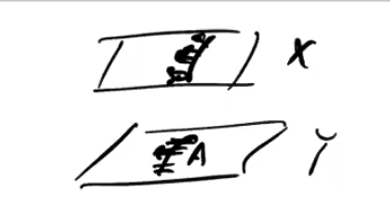
\includegraphics[width=3.64583in,height=\textheight]{figures/image_2020-11-15-01-41-25.png}
\caption{Image}
\end{figure}

\end{remark}

\begin{remark}

There are some equivalent definitions of a morphism being étale:

\begin{itemize}
\item
  Smooth of relative dimension zero
\item
  Locally finite presentation and \emph{formally étale}
\item
  Locally \emph{standard étale}, i.e.~for each \(x\in X\) with
  \(y\da f(x)\), there exists a \(U\ni x, V\ni y\) such that
  \(f(U) \subseteq V\) and \(V=\spec(R), U = \spec\qty{R[x]_h / g}\)
  (where we localize at \(h\)) such that the derivative \(g'\) is a unit
  in \(R[x]_h\) and \(g\) is monic.
\end{itemize}

For this last definition, thinking of \(\spec(R[x])\) as
\(R\times \AA^n\), what happens when modding out by a polynomial \(g\)?
This yields a curve cutting out the roots of \(g\). Inverting \(h\)
deletes the locus where \(h\) vanishes, and \(g'\) being a unit means
that the \(g\) has no double roots in the fibers. In other word, the
deleted locus passes through all double roots:

\begin{figure}
\centering
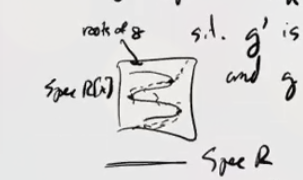
\includegraphics[width=3.64583in,height=\textheight]{figures/image_2020-11-15-01-47-05.png}
\caption{Image}
\end{figure}

\end{remark}

\begin{exercise}[?]

Check that standard étale morphisms are étale, and try to understand the
proof that all étale morphisms are locally standard étale.

\end{exercise}

\begin{example}[Example of an étale morphism]

\envlist

\begin{itemize}
\item
  Multiplication by \([n]\) on an elliptic curve if \(n \in \ZZ\) is
  invertiable in the base field.
\item
  Take \(\GG_m = \spec k[t, t^{-1}]\), and the map
  \begin{align*}  
  \GG_m &\to \GG_m \\
   t^m &\mapsfrom t
  ,\end{align*} where \(n\) is prime to \(\ch(k)\).\footnote{Here we use
    the convention that everything is prime to zero. Also note that this
    map is in fact finite étale.}
\end{itemize}

\end{example}

\begin{exercise}[?]

Show that the last map above is étale.

\emph{(Hint: use the fact that \(\dd{}{t} (t^n) = nt^{n-1}\), which is a
unit.)}

\end{exercise}

\begin{example}[?]

Consider the map
\begin{align*}  
\GG_m &\injects \AA^1 \\
k[t, t^{-1}] &\mapsfrom k[t]
.\end{align*} We need to check 3 things:

\begin{itemize}
\tightlist
\item
  Locally finite presentation,

  \begin{itemize}
  \tightlist
  \item
    This is a finitely presented ring map, since you just need to adjoin
    an inverse of \(t\), one element and one relation.
  \end{itemize}
\item
  Flat,

  \begin{itemize}
  \tightlist
  \item
    Since open embeddings are flat,
  \end{itemize}
\item
  \(\Omega^1_{\GG_m / \AA^1} = 0\),

  \begin{itemize}
  \tightlist
  \item
    True for a Zariski open embedding.
  \end{itemize}
\end{itemize}

Note that this is finite onto its image.

\end{example}

\begin{proposition}[?]

Any open immersion is étale.

\end{proposition}

Note that we actually already checked this!

\begin{example}[An étale morphism that is not finite onto its image]

Use the fact that \(\GG_m\) is \(\AA^1\sm\ts{\vector 0}\), so take
\(\GG_m \sm\ts{1}\) and the map
\begin{align*}  
\GG_m\sm\ts{1} &\to \GG_m \\
t^2 &\mapsfrom t
.\end{align*}

What's the picture? For the squaring map, there are two square roots:

\begin{figure}
\centering
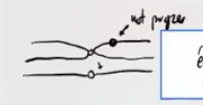
\includegraphics{figures/image_2020-11-15-02-01-04.png}
\caption{Image}
\end{figure}

This is an étale surjection but not finite étale, since it is not
proper. This also gives a counterexample to étale morphisms always
looking like covering spaces, since here that may be true locally but
doesn't hold globally.

\end{example}

\begin{warnings}

This is an important example to keep in mind, because you'll often see
arguments that treat étale maps as though they were finite onto their
image.

\end{warnings}

\begin{example}[?]

Take a finite separable field extension, taking \(\spec\) of it yields
an étale map.

\end{example}

Now for some non-examples:

\begin{example}[A finite map which is not etale]

Take \(X = \spec k[x, y] / xy\), which looks like the following:

\begin{figure}
\centering
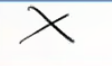
\includegraphics[width=3.64583in,height=\textheight]{figures/image_2020-11-15-02-04-46.png}
\caption{\(X\)}
\end{figure}

Then the normalization \(\tilde X\to X\) is not étale, since it is not
flat.

\end{example}

\begin{example}[A finite flat map which is not etale]

Take the map
\begin{align*}  
\AA^1 &\to \AA^1 \\
t^2 &\mapsfrom t
.\end{align*}

The picture is the following:

\begin{figure}
\centering
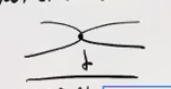
\includegraphics{figures/image_2020-11-15-02-07-04.png}
\caption{Image}
\end{figure}

This is note étale since it is ramified at zero. We can compute
\begin{align*}  
\Omega_f^1 = k[t]\, dt / d(t^2) = k[t] dt/ 2t\, dt
,\end{align*} where \(2t\,dt\) does not generate this module. This is
supported at \(t=0\) if \(\ch \neq 2\).

\end{example}

\begin{example}[?]

A finite flat morphism such that \(\Omega_{X/Y}^1\) is not torsion: a
hint is that the previous example almost works, with a slight
modification. Let \(\ch k = p\), and take
\begin{align*}  
\AA^1 &\mapsvia{F} \AA^1 \\
t^p &\mapsfrom t
.\end{align*} Then \(\Omega_f^1 = k[t]\, dt / d(t^p) = k[t]\,dt\) since
\(d(t^p) = 0\) in characteristic \(p\). This yields line bundles (?), so
it is not torsion.

\end{example}

\begin{remark}

This map has a name: \textbf{the relative Frobenius}. In general,
looking at Frobenii, the Kahler differentials will be very big. You
might not be used to this: in characteristic zero, a map of relative
dimension zero is generically étale. In this case, the Kahler
differentials will always be torsion.

\end{remark}

\begin{example}[?]

Consider a map
\begin{align*}  
\AA^m &\mapsvia{f_1, \cdots, f_m} \AA^m
,\end{align*} since such a map is given by a system of \(m\) polynomials
in \(m\) variables. Then \(f\) is étale is a neighborhood of
\(\vector a\) if \(\det \qty{\dd{f_i}{x_j} \evalfrom_{\vector a} }\) is
a unit.

\end{example}

\hypertarget{properties-of-uxe9tale-morphisms}{%
\subsubsection{Properties of Étale
Morphisms}\label{properties-of-uxe9tale-morphisms}}

\begin{proposition}[Some properties of étale morphisms]

\envlist

\begin{enumerate}
\def\labelenumi{\arabic{enumi}.}
\tightlist
\item
  Open immersions are étale
\item
  Compositions of étale morphisms are étale\footnote{What do you have to
    check? Locally finite presentation, flat, and unramified are all
    preserved. The one that may be tricky is remaining unramified, a
    hint is to use the cotangent exact sequence for \(\Omega^1_{X/Y}\).}
\item
  Base change of étale morphisms are étale, i.e.~

  \begin{center}
  \begin{tikzcd}
  X \cross_Y T\ar[d, "\therefore \text{étale}"']\ar[r] & X\ar[d, "\text{étale}"]  \\
  T\ar[r] &  Y\\
  \end{tikzcd}
  \end{center}
\item
  There is a 2 out of 3 property: If \(\phi \circ \psi\) and \(\phi\)
  are étale, then \(\psi\) is étale.
\end{enumerate}

\end{proposition}

\begin{exercise}[?]

Show property 4 above.

\end{exercise}

\begin{proposition}[?]

Étale morphisms on varieties over an algebraically closed field induce
isomorphisms on complete local rings at closed points.

\end{proposition}

\begin{exercise}[?]

Prove this! Hint: use the criterion for formal étaleness. There's an
evident map one way on local rings coming from your étale morphism, and
you need to produce the inverse map.

\end{exercise}

\begin{exercise}[?]

\(\danger\) If \(\psi\) is étale and \(\phi\circ\psi\) is étale, it is
not necessarily the case that \(\phi\) is étale. Come up with an
example!

\end{exercise}

\begin{corollary}[An informal statement]

Any property that can be checked at the level of complete local rings is
true for the source of an étale morphism if it is true for the target.

\end{corollary}

Why? If you want to check a property for complete local rings on the
source, note that the map induces an isomorphism of complete local
rings.

\hypertarget{generalizing-topologies}{%
\subsection{Generalizing Topologies}\label{generalizing-topologies}}

\hypertarget{sites}{%
\subsubsection{Sites}\label{sites}}

The notion of a \emph{site} will be a generalization of topological
spaces and sheaves. The idea is we'll generalize sheaf cohomology to
this setting. On a nice space like a manifold, singular cohomology is
isomorphic to the sheaf cohomology of the constant sheaf
\(\underline{\ZZ}\). Here we'll find some version of a sheaf where étale
cohomology with \(\ZZ/\ell^n\ZZ\) coefficients will be the sheaf
cohomology with the constant sheaf \(\underline{\ZZ/\ell^n\ZZ}\).

\begin{question}

What parts of the definition of a topological space are needed to define
the notion of a sheaf?

\end{question}

\begin{remark}

Recall that the \emph{sheaf condition} is given in two parts:

\begin{enumerate}
\def\labelenumi{\arabic{enumi}.}
\item
  A section is determined by its value on a cover, and
\item
  Sections can be glued when they agree on intersections.
\end{enumerate}

\end{remark}

\begin{answer}

\envlist

\begin{enumerate}
\def\labelenumi{\arabic{enumi}.}
\tightlist
\item
  As in presheaves, a notion of open sets and inclusions. (I.e., a
  category of open sets.)\footnote{Recall that a presheaf on \(X\) is a
    contravariant functor out of the category of open sets of \(X\).}\footnote{The
    notion of a presheaf on \(X\) doesn't know much about the actual
    topology of \(X\). If two spaces have the coarsest topology, so the
    only opens are \(X, \emptyset\), then the categories of open sets
    are equivalent, and every presheaf on them will be the same.}
\end{enumerate}

We'd also like to make sense of the sheaf condition:

\begin{enumerate}
\def\labelenumi{\arabic{enumi}.}
\setcounter{enumi}{1}
\item
  Collections of morphisms which are ``covers'', remembering which
  collections of opens cover a space, and
\item
  The existence of certain fiber products (intersections).
\end{enumerate}

\end{answer}

\begin{remark}

The motivation for (3) above is that for \(U, V \subseteq X\), we can
form \(U\cross V = U\intersect V\).

\end{remark}

\begin{definition}[Preliminary: Sites/Grothendieck Topologies]

A category \(\mathcal{C}\) with a collection of \emph{covering
families}\footnote{How to think of this: elements in this collection
  cover \(X\).}
\begin{align*}
\ts{X_\alpha \mapsvia{f_\alpha} X \st \alpha\in A}
\end{align*} such that several axioms are satisfied.

\end{definition}

We'll discuss the axioms next time, they just capture the notion of what
a cover of a topological space should look like.

\begin{warnings}

There are at least three different notions of this definition! The one
above is perhaps the least general but the easiest to work with.

\end{warnings}

\begin{example}[?]

For \(X\) a topological space, \(\mathcal{C}\) the category of open sets
in \(X\), then \(\ts{U_\alpha\to U}\) is a covering family if the
\(U_\alpha\) cover \(U\), i.e.~\(U = \union_\alpha U_\alpha\).

\end{example}

\begin{example}[More exotic]

Let \(M\) be a manifold and \(\mathcal{C}\) be the category of manifolds
over \(M\), so all \(M' \mapsvia{f} M\) such that \(f\) is locally an
isomorphism. Note that these are smooth local homeomorphisms. Let
\begin{align*}
\ts{M_\alpha \mapsvia{f_\alpha} M} \text{ if } \Union_\alpha \im (f_\alpha) = M
\end{align*}

\end{example}

\begin{example}[Another exotic example]

Let \(X\) be a scheme and consider \(X_{\text{et}}\) the category of all
étale \(Y/X\): so the objects are schemes \(Y\) admitting an étale
morphism \(Y\to X\). Then \(\ts{X_\alpha\to X}\) is a covering family if
\(\union \im (f_\alpha) = X\).

\end{example}

This will be the fundamental object, and we'll define étale cohomology
by defining sheaves on this category, taking a constant sheaf
\(\underline{\ZZ/\ell^n\ZZ}\), and we'll take sheaf cohomology.

\hypertarget{lecture-3}{%
\section{Lecture 3}\label{lecture-3}}

\hypertarget{defining-sites}{%
\subsection{Defining Sites}\label{defining-sites}}

Today: we'll discuss sites, which generalizes the category of open sets
over a topological space. The goal is to generalize spaces and sheaves
to categories, and to define a sheaf we need

\begin{enumerate}
\def\labelenumi{\arabic{enumi}.}
\item
  A notion of a \emph{cover}, and
\item
  A notion of intersections/fiber products of open sets.
\end{enumerate}

\begin{definition}[Grothendieck Topology / Sites]

A \textbf{Grothendieck topology} on \(\mathcal{C}\) or a \textbf{site}
on \(\mathcal{C}\) is the data of for each
\(X\in \mathrm{Ob}(\mathcal{C})\) a collection of sets of morphism
\(\ts{X_\alpha \to X}\) (\emph{covering families}) satisfying

\begin{itemize}
\item
  Intersections exist: If \(X_\alpha\to X\) appears in a covering family
  and \(Y\to X\) is arbitrary, the fiber product \(X_\alpha\cross_X Y\)
  exists.
\item
  Intersecting with a cover again yields a cover: If
  \(\ts{X_\alpha\to X}\) is a covering family and \(Y\to X\) is
  arbitrary, then the covering family can be pulled back:
  \(\ts{Y\cross_X X_\alpha\to Y}\) is again a covering
  family.\footnote{When \(\mathcal{C}\) was the category of open sets of
    a space \(X\), the existence of this morphism \(Y\to X\) says
    \(Y \subseteq X\) is an open subset, and thus intersecting \(Y\)
    with any open cover of \(X\) yields an open cover of \(Y\).}
\item
  Compositions of coverings are again coverings: If
  \(\ts{X_\alpha\to X}_{\alpha}\) and
  \(\ts{X_{\alpha\beta} \to X_\alpha}_{\alpha,\beta}\) are covering
  families, then you can compose, i.e.~taking the set of all possible
  ways of composing \(\ts{X_{\alpha\beta} \to X_\alpha \to X}\) is again
  a covering family.\footnote{For spaces, this says if you have a cover
    of an open set by subsets and a cover of each of those subsets, the
    entire set has been covered.}
\item
  Isomorphisms are covers: If \(X\mapsvia{\sim_f} Y\) is an isomorphism,
  then the singleton family \(\ts{X\mapsvia{f} Y}\) is a covering
  family.
\end{itemize}

\end{definition}

\hypertarget{examples-of-sites}{%
\subsubsection{Examples of Sites}\label{examples-of-sites}}

\begin{example}[The motivating example]

If \(X\) is a topological space, define \(\mathcal{C}\) whose objects
are open subsets of \(X\) where there is a unique morphism \(U\to V\)
iff \(U\subseteq V\). Then \(\ts{U_\alpha \to U}\) is a covering family
if \(\Union_\alpha U_\alpha = U\).

\end{example}

\begin{example}[The small étale site]

Let \(X\) be a scheme, and define the small étale site \(X_{\et}\): the
category whose objects are étale morphisms \(Y\mapsvia{f} X\) where
morphisms are maps over \(X\):

\begin{center}
\begin{tikzcd}
Y_1 \ar[rd, "{f_1}"]\ar[rr, "g"] & & Y_2\ar[ld, "{f_2}"] \\
 & X & 
\end{tikzcd}
\end{center}

Note that \(g\) is étale by the 2 out of 3 property.

Then \(\ts{X_\alpha\to X}\) is a covering family if the set theoretic
images satisfy \(\Union_\alpha \im(f_\alpha) = X\).

\end{example}

\begin{example}[The big étale site]

Again let \(X\) be a scheme, and define \(X_{\mathrm{Et}}\) the category
whose objects are all \(X\dash\)schemes (where we no longer require the
maps to be étale). In other words, this is the overcategory of \(X\):
the category of schemes over \(X\). Then
\(\ts{U_\alpha\mapsvia{f_\alpha}U}\) is a covering family if all of the
\(f_\alpha\) are étale and \(\Union_\alpha \im(f_\alpha) = U\).

\end{example}

Note the difference: in the small site, we included only étale
\(X\dash\)schemes, vs all \(X\dash\)schemes in the big site. In both
cases, the notion of covering families are the same.

\begin{example}[?]

Let \(X\) be a complex analytic space (e.g.~a complex manifold), then
there is an analytic étale site whose objects are complex analytic
spaces \(Y\mapsvia{f} X\) such that locally on \(Y\), \(f\) is an
analytic isomorphism. Note that this includes covering spaces. The
morphisms will be morphisms over \(X\) creating commuting triangles, and
the covers are the usual covers.

\end{example}

\begin{remark}

This category is part of what motivates the definition of the étale
topology. This is what we're trying to imitate. E.g. if you have a
complex algebraic variety, taking its analytification will be one of
these. This site will show up later when we compare étale cohomology to
singular cohomology.

\end{remark}

\begin{remark}

We haven't said what it means to be a sheaf yet, but Grothendieck
topologies behave in somewhat unexpected ways. The category of sheaves
of the analytic étale cohomology, \(\Sh(X_{\mathrm{an\dash et}})\), is
canonically equivalent to \(\Sh(X^{\mathrm{top}})\). Thus sometimes the
category of sheaves over a site doesn't remember the site, i.e.~two
different sites can have the same category of sheaves. On the RHS we had
a category of open subsets, whereas on the LHS we included things like
covering spaces. We'll see later that there is a notion of morphisms of
sites, and there is a morphism inducing this equivalence.

Proving this isomorphism will be an exercise, here's an outline of why
it's true: suppose you have a cover of \(X\) in this category, i.e.~a
family of local analytic isomorphisms. Given any of these, you can cover
by subsets for which these are isomorphisms onto their images.

\end{remark}

\begin{definition}[fppf]

The letter \textbf{fppf} stand for \textbf{faithfully flat and finite
presentation}. \footnote{The letters don't precisely match up here
  because this comes from a French acronym.}

\end{definition}

\begin{example}[The fppf topology]

There are small and big sites here: we define \(X_{\fppf}\) whose
objects are fppf morphism \(Y\to X\), with morphisms as triangular
diagrams of morphisms over \(X\), and covers are the usual covers. Note
that replacing fppf morphisms with flat morphisms would yield an
equivalent definition here.

\end{example}

\begin{example}[?]

If \(X\) is a scheme, then the small Zariski topology is
\(X_{\mathrm{zar}}\) whose objects are \(\Op(X^{\mathrm{top}})\), the
Grothendieck topology of the corresponding topological space, and we
take the usual notion of covers. There is a big Zariski topology
\(X_{\mathrm{Zar}}\) whose category is all \(X\dash\)schemes
\(\ts{U_\alpha\mapsvia{f_\alpha} U}\) with \(f_\alpha\) open embeddings
and \(\Union_\alpha \im(f_\alpha) = U\).

\end{example}

\begin{example}[?]

Some other examples:

\begin{itemize}
\item
  The \textbf{Nisnevich} topology, which lives between the Zariski and
  the étale topology,
\item
  The \textbf{crystalline} site, used to define crystalline cohomology,
\item
  The \textbf{infinitesimal} site,
\item
  The \textbf{cdh} topology, the \textbf{arc} topology, the \textbf{rh}
  topology, and many more.
\end{itemize}

\end{example}

\hypertarget{toward-sheaves-of-sites}{%
\subsection{Toward Sheaves of Sites}\label{toward-sheaves-of-sites}}

\begin{definition}[Presheaf]

For \(\mathcal{D}\) a category, a \(\mathcal{D}\dash\)valued
\textbf{presheaf} is a contravariant function
\(F:\mathcal{C}\to \mathcal{D}\).

\end{definition}

\begin{remark}

This makes no reference to any Grothendieck topology.

\end{remark}

\begin{example}[?]

If \(X\) is a topological space, a \(\mathcal{D}\dash\)valued presheaf
of \(X\) is equivalent to a presheaf on \(\Op(X)\).

\end{example}

We can now define a sheaf. What's the motivation? For \(X\) a
topological space, it's a sheaf satisfying some conditions: its sections
are determined by an open cover, and given sections agreeing on overlaps
allows gluing. This can be captured by a specific diagram, which is what
we will use here.

Recall that a site is a category equipped with the Grothendieck
topology.

\begin{definition}[Sheaf]

A \textbf{sheaf} \(F\) is presheaf such that

\begin{center}
\begin{tikzcd}
F(U) \ar[r] & \prod_\alpha F(U_\alpha) \ar[r, shift left=0.75ex, "F(\pi_1)"] \ar[r, shift right=0.75ex, "F(\pi_2)"'] & \prod_{\alpha, \alpha'} F(U_\alpha \cross_U U_{\alpha'}) 
\end{tikzcd}
\end{center}

is an \emph{equalizer} diagram for all covering families
\(\ts{U_\alpha \to U}\).

\end{definition}

\begin{remark}

The diagram arises due to the fact that if we have a bunch of maps
coming from a cover, since we have a contravariant functor, we get a map
into the product. We then look at the intersections of all
\(U_{\alpha}, U_{\alpha'}\).

The two arrows occurring come from the projections:

\begin{center}
\begin{tikzcd}
& U_\alpha \cross_U U_{\alpha'} \ar[dl, "\pi_1"] \ar[rd, "\pi_2"] & \\
U_\alpha\ar[dr, hook] & & U_{\alpha'}\ar[dl, hook] \\
& U &
\end{tikzcd}
\end{center}

where we use the fact that since \(F\) is a contravariant functor, it
induces maps going the other way.

What does being an equalizer mean, say if \(F\) is set-valued?
``Exactness'' at the middle term is the gluing condition, and exactness
at the first term is injectivity, i.e.~a section (the values of \(F\) on
\(U\)) are determined by its values on a cover (by \(F(U_\alpha)\)).
Note that in fact \(F(U)\) is the limit of this diagram. The gluing
condition is more precisely that if we're given
\((s_\alpha) \in \prod_\alpha F(U_\alpha)\) such that
\(F(\pi_1)(s_\alpha) = F(\pi_2)(s_\alpha)\), then \((s_\alpha)\) comes
from \(F(U)\).

\end{remark}

\begin{definition}[Morphisms of sheaves and presheaves]

A \textbf{morphism} \(F_1\to F_2\) of either presheaves or sheaves is a
natural transformation of functors.

\end{definition}

\hypertarget{examples-of-sheaves-of-sites}{%
\subsubsection{Examples of Sheaves of
Sites}\label{examples-of-sheaves-of-sites}}

\begin{theorem}[?]

Any representable functor is a sheaf on the étale site \(X_{\Et}\). In
fact, any such functor is a sheaf on the big fppf site \(X_{\Fppf}\):
the category of all \(X\dash\)schemes with covers as fppf covers, which
are maps that are flat and jointly surjective.

\end{theorem}

\begin{example}[Examples of sheaves on the étale site]

Take \(\mu_n\) the functor represented by
\(\mu_n \da \spec k[t] / t^{n-1}\). For \(U\) an \(X\dash\)scheme, we
can evaluate in the following way:
\begin{align*}  
\mu_n(U) = \ts{f\in \OO_U(U) \st f^n = 1}
.\end{align*}

\end{example}

\begin{example}[?]

We define a sheaf of the étale site as \(\OO^{\et}_X(U) = \OO_U(U)\)
where we've said what the values are. This is a sheaf that is
represented by \(\AA^1_{/X}\).

\end{example}

\begin{example}[?]

The constant sheaf \(\underline{\zlnz}\). How can we prove it is a
sheaf, given the theorem, and determine what its values are? This is
represented by \(\qty{\zlnz} \cross X\), i.e.~taking the disjoint union
of \(\ell^n\) copies of \(X\). The values are given by
\begin{align*}  
\underline{\zlnz}(U) =  \hom_{\Top}(U^{\Top}, \zlnz)
,\end{align*} where we give the set \(\zlnz\) the discrete topology and
take morphisms to be continuous maps.

\end{example}

\begin{warnings}

The constant sheaf \(\underline{S}\) doesn't associate \(S\) to every
open set: it instead associates \(S^d\) where \(d\) is the number of
components. The former would only be a presheaf, and not a sheaf.

\end{warnings}

\begin{example}[?]

We can take the sheaf \(\GG_m(U) \da \OO_U(U)\units\), whose values are
obtained by taking the global sections of the structure sheaf and only
keeping the units. This is represented by
\begin{align*}
\GG_{m, X} = \spec \ZZ[t, t^{-1}] \fp{\spec \ZZ} X
\end{align*} Why does this represent this functor? Mapping into this
requires that \(t\) goes to an invertible function, which yields the
isomorphism.

\end{example}

\begin{remark}

Note that all of these functors take values in abelian groups, which is
a consequence of the fact that the representing objects are group
schemes. In fact, one definition of a group scheme is that the functor
it represents factors through groups.

\end{remark}

\begin{example}[?]

Take the functor \(\PP^n(U) \da \hom(U, \PP^n)\). This functor can be
written down as a line bundle on \(U\) with a surjective map from
\(\OO_U \to \OO_U^n\) (?), the functor represented by projective space,
and that's also a sheaf that is necessarily representable but not an
abelian one.

\end{example}

Some things we still need to get to:

\begin{itemize}
\tightlist
\item
  A proof that \(\ul{\zlnz}\) is actually a sheaf,
\item
  A proof that the category of sheaves on the big étale site
  \(X_\Et\)\footnote{Note that a sheaf on the big étale site necessarily
    restricts to a sheaf on the small étale site, since covers in the
    small site are also covers in the big site.} with values in
  \(\thecat{Ab}\) is abelian and has enough injectives.
\end{itemize}

\hypertarget{uxe9tale-cohomology-a-preliminary-definition}{%
\subsection{Étale Cohomology: A Preliminary
Definition}\label{uxe9tale-cohomology-a-preliminary-definition}}

\begin{definition}[Imprecise: étale cohomology]

Let \(\mathcal{F}\) be a sheaf and define a functor
\(\Gamma_X: \mathcal{F}\to \mathcal{F}(X)\) sending it to its values on
\(X\). Then the \textbf{étale cohomology} of \(X\) is defined by
\begin{align*}  
H^i(X_\et, \ul{\zlnz}) \da R^i \Gamma_X(\ul \zlnz)
,\end{align*} the right-derived functors of \(\Gamma_X\).

\end{definition}

\begin{remark}

This definition is incomplete, and in particular, it's highly
non-obvious that this category of abelian sheaves is abelian. E.g.
usually when proving that the category of abelian sheaves on a
topological space has cokernels, you use sheafification: you take the
cokernel of a map of presheaves, which is a presheaf, and sheafify it.
Here, we don't know how to sheafify a presheaf on a site. The usual
construction involves forming the \emph{espace étalé} and taking
sections does not work for a site, you need a genuinely different
argument.

\end{remark}

\begin{warnings}

Even showing cokernels exist in the category of abelian sheaves on a
site is nontrivial. Try as an exercise!

\end{warnings}

\begin{remark}

What will be true in general is that this category will be an \(AB5\)
abelian category, and having enough injectives is all that's
additionally needed. This comes from machinery developed in
Grothendieck's Tohoku paper, and we'll sketch part of the proof.

\end{remark}

Properties of these sheaves are not so obvious, and depend on the site
you're working over:

\begin{example}[?]

Consider the map
\begin{align*}  
\GG_m &\to \GG_m \\
t^m &\mapsfrom t
,\end{align*} where \(n\) is invertible over the base, e.g.~if we're
over a field of characteristic coprime to \(n\). This yields a map of
sheaves in two different settings. In \(X_{\mathrm{Zar}}\) we have
\begin{align*}  
\OO\units &\to \OO\units \\
f &\mapsto f^n
.\end{align*}

We can look at this in \(X_{\et}\), yielding
\begin{align*}  
\OO_\et\units &\to \OO_\et\units \\
f &\mapsto f^m
.\end{align*}

\begin{claim}

This map is not an epimorphism on \(X_{\mathrm{Zar}}\) but is on
\(X_{\et}\)

\end{claim}

\begin{proof}[?]

It suffices to give one example: take \(X = \spec \RR\) and \(n=2\), and
since this is just a point, the sheaf is determined by its values. So is
the map
\begin{align*}  
\RR\units &\to \RR\units \\
t &\mapsto t^2
\end{align*} surjective? The answer is no, of course, since its image is
\(\RR_{\geq 0}\).

This will be surjective on \(X_{\et}\) if \(n\) is invertible on \(X\).
If we were in usual topological spaces, we would want to show that given
any section of the sheaf on an open set, it can be refined. Here we want
to pass to an étale cover so that section has an \(n\)th root. So given
\(f\in \GG_m(U)\), we want an étale cover of \(U\) so that \(f\) obtains
an \(n\)th root. An invertible function is a map \(U\to \GG_m\), and we
can form the square

\begin{center}
\begin{tikzcd}
 U \fp{\GG_m} \GG_m\ar[r]\ar[d] & \GG_m & z^m  \ar[d] \\
 U\ar[r] &  \GG_m & z\ar[u, |->]
\end{tikzcd}
\end{center}

The RHS map is étale since \(n\) is invertible, and the fiber product is
étale since étale morphisms are preserved by base change.

\begin{claim}

\(f\) has an \(n\)th root upstairs. (Verify!)

\end{claim}

There's a more concrete way of writing this: note that
\(\AA^1_{U, z} = \spec k[t]\), so take the subscheme cut out by
\(V(z^n - f)\). This will be an étale cover of \(U\) (the same one in
fact) and \(z\) is now an \(n\)th root.

\end{proof}

\end{example}

\begin{exercise}[?]

Check the details! Namely that this argument implies that this map of
sheaves is an epimorphism.

\end{exercise}

\begin{remark}

This map of sheaves \(\GG_m \mapsvia{z^m \mapsfrom z} \GG_m\), noting
that if \(n\) is not invertible this will not be an epimorphism, will
always be an epimorphism in \(\Sh(X_\fppf)\) since this map is flat and
finitely presented.

\end{remark}

\hypertarget{preview-morphisms-of-sites}{%
\subsection{Preview: Morphisms of
Sites}\label{preview-morphisms-of-sites}}

\begin{definition}[Morphisms of Sites]

Suppose \(T_1, T_2\) are sites (categories with covering families), then
a \textbf{continuous map of sites} \(f:T_1 \to T_2\) is a functor
\(T_2 \to T_1\)\footnote{Note that this functor goes in the opposite
  direction of the original map.} that preserves fiber products and
sends covering families to covering families.

\end{definition}

\begin{example}[?]

A continuous map \(f\in \Hom_\Top(X, Y)\) induces a map
\begin{align*}  
\Op(Y) &\to \Op(X) \\
U &\mapsto f^{-1}(U)
.\end{align*}

\end{example}

\begin{exercise}[?]

Check that this is a continuous map of sites.

\end{exercise}

Next time: a bunch of examples.

\hypertarget{lecture-4-descent}{%
\section{Lecture 4: Descent}\label{lecture-4-descent}}

Last time: sites, sheaves, and morphisms of sites. Today: descent, which
is how we'll see that many familiar objects are sheaves on the étale
site, such as representable functors or quasicoherent sheaves.

\hypertarget{reminder}{%
\subsection{Reminder}\label{reminder}}

\begin{definition}[A continuous map of sites]

Given two sites \((C, T_1)\) and \((D, T_2)\) where \(C, D\) are
categories and the \(T_i\) are collections of covering families, a
\textbf{morphism} is a functor \(f^{-1} :D\to C\) such that

\begin{enumerate}
\def\labelenumi{\arabic{enumi}.}
\tightlist
\item
  \(f^{-1}\) preserves fiber products.
\item
  \(f^{-1}\) sends covering families to covering families.
\end{enumerate}

\end{definition}

\begin{example}[?]

The main example: for \(f:X\to Y\) a map of topological spaces, the
functor \(F: \Op(Y) \to \Op(X)\) given by \(F(U) \da f^{-1}(U)\) sending
an open set to its preimage.

\end{example}

\begin{exercise}[Check!]

Check that this is a continuous map of sites.

\end{exercise}

\begin{example}[?]

Suppose \(X\) is a scheme, then there is a natural map of sites from
\(X_{\Fppf}\) (all \(X\dash\)schemes where covers are collections of
jointly surjective flat morphism) to \(X_{\Et}\) (all \(X\dash\)schemes
where covers are jointly surjective étale morphisms) to \(X_{\et}\)
(étale \(X\dash\)schemes with morphisms over \(X\)) to \(X_{\zar}\) (the
open subsets of \(X\) with morphisms given by inclusions and covers the
usual covers). The maps here are inclusions going the other way.

\end{example}

\begin{exercise}[Check!]

Check that these are continuous maps of sites.

\end{exercise}

\begin{remark}

\envlist

On terminology:

\begin{itemize}
\item
  What we've been calling a site or a Grothendieck topology is sometimes
  called a \emph{Grothendieck pretopology}. The major difference is that
  you don't have to assume the existence of fiber products.
\item
  You may also see the notion of a \textbf{topos}, which is the category
  of sheaves on a site.
\end{itemize}

\end{remark}

\hypertarget{setting-up-descent}{%
\subsection{Setting up Descent}\label{setting-up-descent}}

\begin{question}

\envlist

\begin{enumerate}
\def\labelenumi{\arabic{enumi}.}
\item
  We've said what it means to be a sheaf on a site, how do we check that
  a given functor is a sheaf on \(X_{\et}\) or \(X_{\fppf}\)?
\item
  How do we construct such sheaves?
\end{enumerate}

\end{question}

\begin{theorem}[Ways of constructing sheaves]

\envlist

\begin{enumerate}
\def\labelenumi{\arabic{enumi}.}
\item
  If \(Y\) is an \(X\dash\)scheme (i.e.~a scheme equipped with a map to
  \(X\)) then the functor \(Z \to \hom_X(Z, Y)\) is a sheaf on
  \(X_{\Fppf}, X_{\Et}, X_{\et}\), etc.
\item
  Suppose \(\mathcal{F}\) is a quasicoherent sheaf on \(X\), so
  \(\mathcal{F}\in \qcoh(X)\), the functor of taking global sections:
\end{enumerate}

\begin{center}
\begin{tikzcd}
Z \ar[dd, "f"] &        & \\
               & \ar[r] & \Gamma(Z, f^* \mathcal{F}) \\
X              &
\end{tikzcd}
\end{center}

is a sheaf on \(X_{\Fppf}, X_{\Et}, X_{\et}\), etc.

\end{theorem}

\begin{definition}[$\mathcal{F}^{\et}$]

The sheaf associated to the above functor on \(X_{\et}\) will be denoted
\(\mathcal{F}^\text{étale}\).

\end{definition}

\begin{proof}[of 2]

Suppose we have an fppf cover of \(X\)

\begin{center}
\begin{tikzcd}
U = \disjoint U_i \ar[d] \\
X
\end{tikzcd}
\end{center}

\end{proof}

\begin{question}

Suppose \(\mathfrak{F}\in \qcoh(X)\). When does it come from a
quasicoherent sheaf on \(X\)? I.e., when is there a quasicoherent sheaf
\(\mathcal{F}'\) on \(X\) and an isomorphism between its pullback to
\(U\) and \(\mathcal{F}\)? What extra structure do you need to
``descend'' to \(\qcoh(X)\), i.e.~to pick such an isomorphism?

\end{question}

\begin{question}

Given \(\mathcal{F}_1, \mathcal{F}_2 \in \qcoh(U)\) and a morphism
\(f: \ro{\mathcal{F}_1}{U} \to \ro{\mathcal{F}_2}{U}\), when does \(f\)
come from \(X\)?

\end{question}

\begin{remark}

If \(X = \spec k\) and \(U\) is a finite separable extension, then this
question is exactly what Galois descent is about!

\end{remark}

\begin{example}[(a motivating one)]

\(U = \disjoint U_i \to X\) is a Zariski cover. If we have a sheaf on
\(U\), what extra data do we need to get a sheaf on \(X\)? We need
isomorphisms
\(\ro{\mathcal{F}_i }{U_i\intersect U_j} \mapsvia{\sim} \ro{\mathcal{F}_j}{U_i\intersect U_j}\)
(gluing data) where each \(\mathfrak{F}_i\) is the sheaf given on
\(U_i\). We also need a cocycle condition on triple intersections. Given
this data, gluing yields a sheaf on \(X\). This may be familiar from
vector bundles. Thus to give a sheaf, it suffices to specify gluing
data.

Morphisms \(\mathcal{F}\to \mathcal{G}\) is the same as morphisms
\(\ro{\mathcal{F}}{U_i} \to \ro{\mathcal{G}}{U_i}\) which commute with
the gluing data. We'd like to generalize this notion of commuting with
gluing data to more general types of covers.

\end{example}

\begin{definition}[Descent data for quasicoherent sheaves]

Suppose \(U\mapsvia{f}X\) is a morphisms, then \textbf{descent data} for
a quasicoherent sheaf on \(U/X\) is the following:

\begin{enumerate}
\def\labelenumi{\arabic{enumi}.}
\tightlist
\item
  A sheaf \(\mathcal{F}\in \qcoh(U)\).
\item
  Gluing data: If we take the fiber product of \(U\) with itself,
  mapping to \(U\) under 2 different projections\footnote{If \(U\) was
    an open cover, this would correspond to intersections of elements in
    the cover.},
\end{enumerate}

\begin{center}
\begin{tikzcd}
U \cross_X U \ar[d, bend left, "\pi_1"] \ar[d, bend right, "\pi_2"'] \\
U
\end{tikzcd}
\end{center}

there are isomorphisms
\begin{align*}  
  \phi: \pi_1^* \mathcal{F} \mapsvia{\sim} \pi_2^* \mathcal{F}
  .\end{align*}

\begin{enumerate}
\def\labelenumi{\arabic{enumi}.}
\setcounter{enumi}{2}
\tightlist
\item
  Cocycle condition: in the following fiber product

  \begin{center}
  \begin{tikzcd}
  U \cross_X U \cross_X U 
  \ar[d, shift  left=1.75ex] \ar[d] \ar[d,shift  right=1.75ex,  "\pi_{ij}"'] \\
  U\cross_X U
  \end{tikzcd}
  \end{center}

  we have \(\pi_{23}^* \phi \circ \pi_{12}^* \phi = \pi_{13}\phi\).
\end{enumerate}

\end{definition}

\begin{exercise}[?]

Check that this agrees with the previous notions when \(U\to X\) is a
Zariski cover.

\end{exercise}

\begin{definition}[Morphisms of descent data]

Given descent data \((\mathcal{F}, \phi)\) and \((\mathcal{G}, \psi)\),
a \textbf{morphism} is a morphism \(h: \mathcal{F} \to \mathcal{G}\) of
quasicoherent sheaves on \(U\) such that the following diagram commutes:

\begin{center}
\begin{tikzcd}
\pi_1^* \mathcal{F} 
\ar[r, "\pi_1^*h"] 
\ar[d, "\phi"'] 
& \pi_1^* \mathcal{G} \ar[d, "\psi"] \\
\pi_2^* \mathcal{F} \ar[r, "\pi_2^*h"'] 
& \pi_2^* \mathcal{G} 
\end{tikzcd}
\end{center}

\end{definition}

\hypertarget{descent-data-is-equivalent-to-quasicoherent-sheaves}{%
\subsection{Descent Data is Equivalent to Quasicoherent
Sheaves}\label{descent-data-is-equivalent-to-quasicoherent-sheaves}}

\begin{theorem}[Descent for quasicoherent sheaves]

Suppose \(f: U\to X\) is fppf. Then \(f^*\) induced an equivalence of
categories between \(\qcoh(X)\) and descent data on \(U/X\).

\end{theorem}

\begin{remark}

This doesn't quite make sense, since we haven't covered how to get
descent data from a given sheaf. Explicitly, given
\(\mathcal{F}\in \qcoh(X)\), we can pullback to obtain
\(f^* \mathcal{F}\in \qcoh(U)\). We now want an isomorphism
\begin{align*}  
\qty{f\circ \pi_1}^* \mathcal{F} \mapsvia{\sim} \qty{f\circ \pi_2}^* \mathcal{F}
\end{align*} on \(U\cross_X U\). We have a situation like the following:

\begin{center}
\begin{tikzcd}
U\cross_X U 
 \ar[r, shift right=0.75ex, "\pi_2"'] \ar[r, shift left=0.75ex, "\pi_1"] 
& U
  \ar[r, "f"] 
& X
\end{tikzcd}
\end{center}

Since \(f\circ \pi_1 = f\circ \pi_2\) in this case, pulling back the
identity yields the desired isomorphism.

\end{remark}

\begin{example}[?]

Let \(U = \disjoint U_i\) be a Zariski cover of \(X\), then vector
bundle can be obtained from \(\OO_{U_i}^{\oplus n}\in \qcoh(U_i)\). To
glue this to a vector bundle on \(X\), we need isomorphism
\(\phi_{ij} \OO_{U_i\intersect U_j}^{\oplus n} \mapsvia{\sim } \OO_{U_i\intersect U_j}^{\oplus n}\)
such that
\(\ro{\phi_{jk}}{U_i \intersect U_j \intersect U_k} \circ \ro{\phi_{ij}}{U_i \intersect U_i \intersect U_k} = \ro{\phi_{ik}}{U_i\intersect U_j \intersect U_k}\).
For \(n=1\), this is gluing data for a line bundle.

\end{example}

\begin{example}[?]

Suppose \(L/k\) is a Galois extension with Galois group \(G\), then
\(\spec L \to \spec k\) is an étale cover. Descent data on this map is a
quasicoherent sheaf on \(\spec L\), i.e.~an \(L\dash\)vector space
\(V\), with an isomorphism \(\pi_1^* V \mapsvia{\phi \sim}\pi_2^* V\)
satisfying the cocycle condition. We can compute
\begin{align*}
\spec L \times_{\spec k} \spec L = \spec L\tensor_k L = \disjoint_{L\mapsvia{\sim} L} \spec L
,\end{align*} which is a torsor for the Galois group, and in fact is
equal to \(\disjoint_{\Gal(L/k)} \spec L\).

\end{example}

\begin{exercise}[?]

Convince yourself that descent data here is the same as Galois descent,
i.e.~a semilinear action.

\emph{(Hint: you will need to use \(\phi\).)}

\end{exercise}

Explicitly, the theorem says

\begin{itemize}
\item
  Given a morphisms of descent data, we get a unique morphism of sheaves
  (fully faithful)
\item
  If you have descent data, it comes from a sheaf (essentially
  surjective)
\end{itemize}

So we need to prove

\begin{enumerate}
\def\labelenumi{\arabic{enumi}.}
\item
  \(f^*\) is fully faithful, inducing an isomorphism on hom sets, and
\item
  \(f^*\) is essentially surjective.
\end{enumerate}

\begin{quote}
Reference: Neron modules by BLR.
\end{quote}

\hypertarget{proof-of-theorem}{%
\subsubsection{Proof of Theorem}\label{proof-of-theorem}}

Given \(\mathcal{F}_1, \mathcal{F}_2 \in \qcoh(X)\), then we have a
functor and thus a map
\begin{align*}
\hom_X(\mathcal{F}_1, \mathcal{F}_2) \mapsvia{f^*} \hom_U(f^*\mathcal{F}_1, f^*\mathcal{F}_2)
\end{align*} We're not trying to show this map is a bijection, since we
need more than that: the morphism should commute with the descent data.
We can produce two maps to fill in the following diagram:

\begin{center}
\begin{tikzcd}
 & & \hom_{U\cross_X U} 
\qty{ (f\circ \pi_1)^* \mathcal{F}_1, (f\circ \pi_1)^* \mathcal{F}_2 }
\ar[dd, equal]\\
\hom_X(\mathcal{F}_1, \mathcal{F}_2)  
\ar[r, "{f^*}"]  &
\hom_U(f^*\mathcal{F}_1, f^*\mathcal{F}_2)
\ar[ru, "\pi_1^*"]
\ar[rd, "\pi_2^*"] 
& \\
 & & \hom_{U\cross_X U} \qty{ (f\circ \pi_2)^* \mathcal{F}_1, (f\circ \pi_2)^* \mathcal{F}_2   } \\
\end{tikzcd}
\end{center}

where these hom sets are equal since \(f\circ \pi_1 = f\circ \pi_2\).

\begin{claim}

Given \(g\in \Hom_U(f^* \mathcal{F}_1, f^* \mathcal{F}_2)\), this is a
morphism of descent data if maps to the same element under \(\pi_1^*\)
and \(\pi_2^*\) using the above identification of hom sets.

\end{claim}

\begin{exercise}[?]

This follows from definitions, check that it holds.

\end{exercise}

Being fully faithful is the same as the above diagram being a equalizer.
I.e., the first map \(f^*\) is injective, yielding faithfulness, and
fullness means that any map in the middle that has the same image under
the two arrows \(\pi_1^*, \pi_2^*\) comes from an element in
\(\hom_X(\mathcal{F}_1, \mathcal{F}_2)\).

Assuming that this is fully faithful, why do quasicoherent sheaves give
sheaves on \(X_{\et}\) or \(X_{\fppf}\)? Being a sheaf was characterized
by an equalizer diagram gotten by replacing the first hom with taking
global sections of \(\mathcal{F}\) on \(X, U, U\cross_X U\).

\begin{remark}

Taking \(\mathcal{F}_1 = \OO\) and \(\mathcal{F}_2 = \mathcal{F}\), this
shows that \(\mathcal{F}^{\et}\) (resp. \(\mathcal{F}^{\fppf}\)) is a
sheaf. In this case, the first hom is global sections of \(\mathcal{F}\)
on \(X\), the middle are global sections of \(\mathcal{F}\) on \(U\),
and the two maps are to the double intersections.

\end{remark}

To prove this is an equalizer diagram, we'll need a lemma:

\begin{lemma}[?]

Suppose \(R\to S\) is a faithfully flat ring morphism (flat and
morphisms on spec are surjective) and suppose \(N\in \rmod\). Then there
is an equalizer diagram

\begin{center}
\begin{tikzcd}
N \ar[r] & N\tensor_R S \ar[r, bend left, "\id_N \tensor \id_S \tensor 1"] \ar[r, bend right, "\id_N \tensor 1 \tensor \id_S"'] & N\tensor_R S \tensor_R S \\
n \ar[r] & n\tensor 1 
\end{tikzcd}
\end{center}

\end{lemma}

This is the case where \(\mathcal{F}_1 = \OO\) and
\(\mathcal{F}_2 = \tilde N\) the quasicoherent sheaf associated to
\(N\), \(U = \spec S \to X = \spec R\).

\begin{proof}[of lemma]

\textbf{Step 1}: (Amazing trick) WLOG \(R\to S\) splits, so there's a
map \(S\to R\) such that \(R\to S\to R\) is the identity. We can tensor
with \(S\), i.e.~push out this map along itself to obtain

\begin{center}
\begin{tikzcd}
R \ar[d]\ar[r] & S \ar[d, "1\tensor \id_S"'] \\
S \ar[r] & S\tensor_R S  \ar[u, bend right, "\exists m"']
\end{tikzcd}
\end{center}

where \(m\) is a section given by multiplication.

\begin{claim}

The claim is that we can replace \(R\) with \(S\) and \(S\) with
\(S\tensor_R S\).

\end{claim}

\begin{proof}[of claim]

Checking the equalizer diagram is the same as showing that the following
sequence is exact:
\begin{align*}  
0 \to N \to N\tensor_R S \mapsvia{f-g} N\tensor_R S\tensor_R S
,\end{align*} where \(f, g\) are the maps given in the equalizer. It
suffices to do this after tensoring with \(S\), since a sequence of
\(R\) modules is exact iff it is exact after tensoring with \(S\). One
direction is easy, since \(S\) is flat, and the other direction follows
from the fact that you can check on each stalk, and after tensoring the
stalks are the same. This requires checking for each point on
\(\spec R\) that the map on stalks is exact, but that's true because we
have a surjective map and this can be checked upstairs.

\end{proof}

\textbf{Step 2}: Suppose \(R\mapsvia{f} S\) splits via a map
\(S\mapsvia{r} S\). The geometric picture is that we're supposing we
have a section to \(U\to X\), and descending amounts to pulling back
along the splitting. We first want to check that \(N\to N\tensor_R S\)
is injective, which is true since we can use the map \(\id_N \tensor r\)
to produce a splitting. Why is this true? Supposing \(n\in N\) maps to
zero, then noting that \(N\to N\tensor_R S \to N\) is the identity and
thus maps \(f(n)\mapsvia{\id} 0\), forcing \(n=0\).

We now want to show exactness in the middle. Define
\begin{align*}
\tilde r: S\tensor_R S &\to S \\
s_1 \tensor s_2 &\mapsto s_1 \cdot f(r(s_2))
\end{align*} Suppose we have something in the image of the differential.
This yields
\begin{align*}  
\id_N \tensor \tilde r \qty{n\tensor s\tensor 1 - n\tensor 1 \tensor s}
= n\tensor s - n\tensor f(r(s))
= n\tensor s - nr(s) \tensor 1
.\end{align*}

Thus \(n\tensor s\tensor 1 - n\tensor 1\tensor s = 0\), putting this in
the kernel of the differential, making the last term above equal to
zero, and thus \(n\tensor s = n r(s) \tensor 1\), which is in the image
of the differential. So anything in the kernel is in the image, where
we've proved it for pure tensors, and it's an exercise to do it in
general.

\end{proof}

\begin{remark}

Given \(R\to S\) faithfully flat, you can define the \textbf{Amitsur
complex}:
\begin{align*}  
N \to N\tensor S \to N\tensor S^{\tensor 2} \to \cdots \to N\tensor S^{\tensor r}
,\end{align*} where the maps are given by alternating sums of identities
with a 1 in the \(i\)th spot. There is a theorem that this is always
exact, essentially by the same proof as above: reduce to the case where
you have a section by tensoring with \(S\), then use the section to
build a nullhomotopy.

\end{remark}

\begin{quote}
Next time: we'll complete the proof of fppf descent.
\end{quote}

\hypertarget{lecture-5}{%
\section{Lecture 5}\label{lecture-5}}

Last time: we started fppf descent, and wanted to show the quasicoherent
sheaves and representable functors give sheaves on \(X_{\et}\) and
\(X_{\fppf}\). Given a quasicoherent sheaf, we take the associated
presheaf on the étale site given by taking the values of its pullback to
any object on the étale site. This yields a sheaf on the étale site, and
we'll also conclude that representable functors yield such sheaves as
well.

\hypertarget{continuation-of-proof}{%
\subsection{Continuation of Proof}\label{continuation-of-proof}}

Reminder of the theorem (fppf descent for quasicoherent sheaves): If
\(f:U\to X\) is an fppf cover, so finitely presented and faithfully
flat, then the pullback \(f^*\) induces an equivalence of categories
\(\Qcoh(X)\) to descent data for quasicoherent sheaves relative to
\(U/X\). This descent data is a quasicoherent sheaf on \(U\), so you can
take its 2 pullbacks to \(U\cross_X U\) (thinking of these as the double
intersections of objects in the cover) which admit an isomorphism
between them which needs to satisfy a cocycle condition on
\(U\cross_X U \cross_X U\). For Zariski covers, this reduces to having a
cover by opens, a sheaf on each objects, and gluing data that satisfies
the usual cocycle condition.

The goal was to prove (1) this functor is fully faithful, so the map on
hom sets is a bijection. Given
\(\mathcal{F}_1, \mathcal{F}_2 \in \qcoh(X)\), we wanted a certain
diagram to be an equalizer. Faithfulness is the injectivity of the first
map \(f^*\), and fullness is showing that elements go to the same place
in the next two maps.

We proved a lemma: if \(R\to S\) is a faithfully flat ring map and
\(M\in \rmod\) then

\begin{center}
\begin{tikzcd}
N\ar[r] & N\tensor S\ar[r] & N\tensor S \tensor S \\
n \ar[r] & n\tensor 1 & \\
 & n\tensor s \ar[r] & n\tensor s \tensor 1
\end{tikzcd}
\end{center}

is an equalizer diagram. We used one of Daniel's favorite tricks in fppf
descent: producing a section by base-changing to \(S\).

\hypertarget{proof-of-full-faithfulness}{%
\subsubsection{Proof of Full
Faithfulness}\label{proof-of-full-faithfulness}}

\begin{exercise}[Step 1, Important]

\textbf{Step 1}: Reduce to the case where \(U\to X\) is affine.

\emph{(Hint: See chapter 6 of Neron models. This will use that the map
has finite presentation, and in fact even less, that the map is
quasicompact.)}

\end{exercise}

\textbf{Step 2}: We now have \(R\to S\) faithfully flat, where we're
thinking of \(U = \spec S, X = \spec R\). Since \(N, M \in \rmod\),
after replacing symbols, we want the following diagram to be an
equalizer:

\begin{center}
\begin{tikzcd}
\hom_R(M, N) \ar[r] &
\hom_S(M\tensor S, N\tensor S) \ar[r, shift left=0.75em]\ar[r, shift right=0.75em] &
\hom_{S\tensor S}(M\tensor S^{\tensor 2}, N\tensor S^{\tensor 2})
\end{tikzcd}
\end{center}

where all tensors are over \(R\). The first map takes a map \(f:M\to N\)
and composes with the map \(N\to N\tensor S\) from the lemma to get a
map \(M\to N\tensor S\), which automatically extends to a map
\(M\tensor S \to N\tensor S\). Exactness in the middle also comes from
the lemma. Alternatively, injectivity of the first map follows from
injectivity of \(N\to N\tensor S\) and left-exactness of
\(\hom(M, \wait)\), as does exactness everywhere else.

A short diversion:

\begin{corollary}[of proof]

For \(\mathcal{F}\in \qcoh(X)\), we defined
\(\mathcal{F}^{\et} \in \presh(X_{\et})\) where
\(\mathcal{F}^{\et}(U\mapsvia \pi X) \da \pi^* \mathcal{F}(U)\) is a
sheaf on \(X_{\et}\) and \(X_{\fppf}\)

\end{corollary}

\begin{proof}[?]

We want to show that if \(U\to V\) is an étale cover, we want

\begin{center}
\begin{tikzcd}
\mathcal{F}(V) \ar[r] &
\mathcal{F}(U) \ar[r, shift right=0.75ex] \ar[r, shift left=0.75ex] &
\mathcal{F}(U\cross_V U) 
\end{tikzcd}
\end{center}

to be an equalizer diagram -- but this is exactly the previous diagram
where \(\mathcal{F}\da \OO\) and \(\mathcal{F}_2 \da \mathcal{F}\).

\end{proof}

\begin{example}[?]

We have an étale sheaf
\(\OO_{X}^{\et}: (U\to X) \mapsto \Gamma(U, \OO_U)\).

\end{example}

\hypertarget{proof-of-essential-surjectivity}{%
\subsubsection{Proof of Essential
Surjectivity}\label{proof-of-essential-surjectivity}}

We have \(U\mapsvia f X\) an fppf cover and descent data
\((\mathcal{F}, \phi)\) on \(U/X\) where \(\mathcal{F}\) is a
quasicoherent sheaf on \(U\) and \(\phi\) is an isomorphism between its
two pullbacks to \(U\cross_X U\) satisfying the cocycle condition on
\(U\cross_X U \cross_X U\). We want some \(\mathcal{G} \in \qcoh(X)\)
such that the pullback admits an isomorphism
\(f^* \mathcal{G} \mapsvia{\sim}\mathcal{F}\) for which the canonical
descent data on the pullback agrees.

We'll use a similar trick to construct \(\mathcal{G}\).

\begin{exercise}[Important]

\textbf{Step 1}: We'll reduce to the case of an affine morphism.

\end{exercise}

\textbf{Step 2}:

Let \(R\mapsvia f S\) and \(M\in \mods{S}\). We'll want an isomorphism
\(\phi: M\tensor_R S\to S\tensor_R M\) of \(S\tensor_R S\) modules
satisfying the cocycle condition. We make the following construction:

\begin{center}
\begin{tikzcd}
M \ar[r, shift left=2.5, "m\mapsto 1\tensor m"] \ar[r, shift right=2.5, "m\mapsto \phi(m\tensor 1)", swap] & S\tensor M \\
\end{tikzcd}
\end{center}

Suppose that \(M\) is of the form \(N\tensor S\) for \(N\in \rmod\), how
would the descent of \(M\) fit into this diagram and relate to these two
maps? Just set \(K\) to be the equalizer of this diagram, i.e.~the
subset of \(M\) that go to the same thing under both maps.

\begin{claim}

There is obvious map \(K\tensor_R S\to M\) since \(K \subseteq M\) and
\(M\in \mods{S}\), so you can include \(K\injects M\) and multiply by
elements of \(S\). Moreover, this map is an isomorphism. Given this
isomorphism, one obtains compatible descent data on \(M\).

\end{claim}

From the lemma, we have an equalizer

\begin{center}
\begin{tikzcd}
R \ar[r] &
S \ar[r, shift right=0.75ex] \ar[r, shift left=0.75ex] &
S\tensor_R S
\end{tikzcd}
\end{center}

to which we can apply \(\wait \tensor_S M\) to obtain

\begin{center}
\begin{tikzcd}
K \ar[r] &
M\tensor S \ar[r, shift right=0.75ex] \ar[r, shift left=0.75ex] &
M\tensor_R S &
\end{tikzcd}
\end{center}

where \(K\) is by definition the above kernel. We want to check that the
map \(K\to M\) appearing here induces an isomorphism
\(K\tensor S \to M\).

\begin{exercise}[Important]

This is true if \(R\to S\) has a section, show this. Given
\(U\mapsvia f X\) with a section \(s\) and \(\mathcal{F}\in \qcoh(U)\)
with descent data, we want \(\mathcal{G}\) such that
\(f^* \mathcal{G} = \mathcal{F}\). You can take
\(\mathcal{G}\da s^* \mathcal{F}\); check that this works.

\end{exercise}

In general, we want to show \(K\tensor S \to M\) is an isomorphism, and
we want to reduce to the case where we have a section. After applying
\(\wait \tensor S\), \(R\to S\) acquires a section. Why? We get a map
\(S\to S\tensor_R S\), and there's a reverse map \(S\tensor_R S\to S\)
given by multiplication. So \(K\tensor S \tensor S \to M\tensor S\) is
an isomorphism, which implies \(K\tensor S\to M\) is an isomorphism due
to the fact that \(S\) is faithfully flat over \(R\) which allows us to
check exactness before or after tensoring with \(S\).

\begin{quote}
The exercises here are among the most important in the course! Totally
necessary to do them.
\end{quote}

\hypertarget{representable-functors}{%
\subsection{Representable Functors}\label{representable-functors}}

\begin{theorem}[?]

Suppose \(p:U\to X\) is an fppf cover. Then the functor
\(p^*: \Sch/X \to\) descent data for schemes on \(U/X\) is fully
faithful (but not an equivalence of categories).

\end{theorem}

\hypertarget{proof-of-theorem-1}{%
\subsubsection{Proof of Theorem}\label{proof-of-theorem-1}}

\begin{exercise}[Step 1]

Reduce to the case where \emph{everything} is affine, including
\(U, X\), and the scheme over \(X\). However, it's enough to reduce to
the case of affine schemes over \(X\), and \(U, X\) are not necessarily
affine.

\end{exercise}

\textbf{Step 2}: If \(Y,Z\) are schemes over \(X\), we want to show the
following is an equalizer diagram:

\begin{center}
\begin{tikzcd}
\hom_X(Y, Z) \ar[r] &
\hom_U(p^* Y, p^* Z) \ar[r, shift right=0.75ex] \ar[r, shift left=0.75ex] &
\hom_{U\cross_X U}(\pi^* p^* Y, \pi^* p^* Z)
\end{tikzcd}
\end{center}

Here we've suppressed the indices on the \(\pi_i\) since their images
are canonically identified. Injectivity is obvious, using that \(U\) is
surjective, two different morphisms of schemes pulled back along a
faithfully flat morphisms are distinct, although we'll prove this. The
real content is that any morphism on \(U\) that maps to the same thing
on \(U\cross_X U\) comes from \(X\), so we can descend morphisms and the
morphisms form a sheaf (which is what we're trying to prove).

We'll deduce this from what we proved about quasicoherent sheaves. By
the first reduction, we can assume \(Y = \underline{\spec}_X \OO_Y\) is
a relative spec, as is \(Z = \underline{\spec}_X \OO_Z\) where the
\(\OO\) here are quasicoherent sheaves of algebras. These are obtained
by taking the pushforward of the structure sheaf along
\(Y\to X, Z\to X\). Rewriting the diagram, the homs are now in the
category of quasicoherent algebras and we have

\begin{center}
\begin{tikzcd}
 \hom(\OO_Z, \OO_Y)\ar[r] &
 \hom(p^* \OO_Z, p^* \OO_Y) \ar[r, shift right=0.75ex] \ar[r, shift left=0.75ex] &
 \cdots
\end{tikzcd}
\end{center}

where we want this to be an equalizer. This is true because the first
map is injective even when ignoring the algebra structure, just looking
at a map of quasicoherent sheaves, we know this is injective. If we have
an element in the middle that is a morphism of algebras mapping to the
same thing, it comes from a quasicoherent sheaf in the first slot. That
this is also a map of quasicoherent algebras follows from the fact that
descent is functorial. A map of algebras is commuting with a bunch of
maps of quasicoherent sheaves, which we know is true on the RHS and is
thus true on the LHS since pullback yields an equivalence of categories.

\hypertarget{consequences}{%
\subsubsection{Consequences}\label{consequences}}

\begin{corollary}[?]

If \(Z \in \Sch/X\), the \(\hom(\wait, Z)\) is a sheaf on
\(X_{\fppf}, X_{\et}, X_{\Et}\), etc.

\end{corollary}

\begin{remark}

\(p^*\) is not essentially surjective in general for schemes. Descent
data for schemes relative to an étale cover \(U/X\) is called an
\textbf{algebraic space}. Note that some definitions may also required
separatedness. When pullback does yield an equivalence of categories,
this is referred to as \textbf{effective descent}.

It \emph{is} essentially surjective for affine schemes and polarized
schemes: if you have descent data for a scheme on \(U/X\) with an ample
line bundle (which also has descent data) then you can descend the
scheme. Thus projective varieties can be descended, provided you also
descend them with an ample line bundle. Replacing \(\spec\) with
\(\proj\) is one way to show this.

\end{remark}

\begin{example}[of sheaves]

\envlist

\begin{itemize}
\tightlist
\item
  \(\GG_m: U \to \OO_U(U)\units\)
\item
  \(\mu_\ell: U\to \ts{f\in \OO_U(U) \st f^\ell = 1}\).
\item
  \(\underline{\zlz}: U\to \hom_{\Top}(U, \zlz)\) sending \(U\) to
  continuous maps from \(U\) to the constant scheme \(\zlz\), i.e.~the
  \(\ell\dash\)points.
\item
  \(\Hilb^{p(t)}(\PP^n)\) Hilbert schemes of projective space. We know
  this is a scheme, so the functor it represents is a sheaf.
\item
  \(\PP^n\), which represents a line bundle with a surjective map from
  the trivial bundle of rank \(n+1\)
\end{itemize}

\end{example}

\begin{exercise}[?]

Work out Galois descent from this point of view.

\end{exercise}

\hypertarget{uxe9tale-cohomology}{%
\subsection{Étale Cohomology}\label{uxe9tale-cohomology}}

What missing ingredients do we need to define cohomology for these
abelian sheaves?

\begin{enumerate}
\def\labelenumi{\arabic{enumi}.}
\tightlist
\item
  We want to show that the category of abelian sheaves on \(X_{\et}\) is
  abelian.
\item
  We need enough injectives.
\end{enumerate}

\begin{remark}

Both of these facts are true for the category of abelian sheaves on
\emph{any} site, i.e.~any category with a Grothendieck topology.

\end{remark}

The proof of (2) will be relatively easy, but the crucial ingredient for
(1) will be the following:

\begin{theorem}[?]

Let \(\tau\) be a site. Then the forgetful functor
\(\Sh(\tau) \to \Presh(\tau)\) has a left adjoint which we'll call
\textbf{sheafification}.

\end{theorem}

We'll just prove this for \(\tau = X_{\et}\). The general theorem is
much longer!

\hypertarget{preliminaries}{%
\subsubsection{Preliminaries}\label{preliminaries}}

Some operations we can do with sheaves:

\hypertarget{pushforward-and-pullback}{%
\paragraph{Pushforward and pullback}\label{pushforward-and-pullback}}

Suppose \(f:\tau_1 \to \tau_2\) to be a continuous morphism of sites,
i.e.~a functor \(f^{-1} : \tau_2 \to \tau_1\) which preserves fiber
products (preserving intersections and covering families).

\begin{definition}[Pushforwards]

Given \(\mathcal{G}\in \Sh(\tau_1)\), define
\(f_* \mathcal{G}\in \Sh(\tau_2)\) by
\begin{align*}  
\qty{f_* \mathcal{G}}(U) \da \mathcal{G}( f^{-1}(U))
.\end{align*}

\end{definition}

Note that this is the usual formula for pushforwards.

\begin{exercise}[Important, must do]

Show that \(f_* \mathcal{G}\) is a sheaf.

\end{exercise}

\hypertarget{lecture-6-filling-in-gaps-uxe9tale-cohomology}{%
\section{Lecture 6: Filling in Gaps, Étale
Cohomology}\label{lecture-6-filling-in-gaps-uxe9tale-cohomology}}

\begin{remark}[A technical point]

Last time a theorem was stated that pullback induced an equivalence of
categories
\(\Qcoh(X_{\zar}) \mapsvia{\sim} \QCoh(X_{\et}) \mapsvia{\sim} \QCoh(X)(X_{\fppf})\);
note that these are the little sites. What about the big sites? There
are similar equivalences between the three corresponding big sites, but
in general, \(\Qcoh(X_{\Zar}) \neq \QCoh(X_{\zar})\).

For example, a quasicoherent sheaf on the big Zariski site is a
quasicoherent sheaf on every \(X\dash\)scheme and morphisms between
various pullbacks. This isn't as affected by what sheaf you have on
\(X\) itself.

\end{remark}

\begin{remark}

Étale descent data for schemes is not quite the same as an algebraic
space: it yields an algebraic space, but the data is not literally the
same.

\end{remark}

\hypertarget{gaps}{%
\subsection{Gaps}\label{gaps}}

\begin{claim}

The category of abelian sheaves on the \(X_{\et}\) is an abelian
category with enough injectives.

\end{claim}

With this in hand, we can use the formalism of derived functors to
define étale cohomology:

\begin{definition}[Étale Cohomology]\label{def:etale_cohomology}

\begin{align*}  
H^i(X_\et, \zlz) \da R^i \Gamma(X_\et, \underline{ \zlz} )
.\end{align*}

\end{definition}

The crucial ingredient (mentioned last time) is the following:

\begin{theorem}[Sheafification for Sites]

For \(\tau\) a site, the forgetful functor
\(\Sh(\tau) \to \presh(\tau)\) has a left adjoint
(\textbf{sheafification}).

\end{theorem}

We'll prove this for the étale site, just Google ``sheafification for
sites'' to find more general proofs. Note that this is actually the
inclusion of a full subcategory. Before the proof, we'll need a few
operations in order to imitate the usual proof that sheafification
exists for usual sheaves. This is done by constructing the \emph{espace
étalé} out of the stalks and define the sheafification to be sections.
The operations we'll need are:

\hypertarget{pushforwards}{%
\subsubsection{Pushforwards}\label{pushforwards}}

For \(f: \tau_1 \to \tau_2\) a continuous map of sites, this was a
reversed functor preserving fibers products and covering families. For
\(\mathcal{G}\in \Sh(\tau_1)\) we constructed \(f_* \mathcal{G}\), and
the exercise was to show that this is a sheaf.

\begin{example}[?]

Let \(f:X\to Y\) be a map of schemes, this induces a map
\(f: X_\et \to Y_\et\) where each \(U/Y\) comes from \(U\cross_Y X\)
over \(X\).

\end{example}

\begin{example}[?]

Suppose \(k=\bar k\) is a field and we have
\(\iota_{\bar X}:\spec k\to X\). We have
\(\Sh\qty{\qty{\spec k}_{\et}} = \Set\), since an étale cover of
\(\spec k\) is a disjoint union of copies of itself. If you show what
the value of a sheaf on \(\spec k\), you know it on any disjoint union
of them since there are a lot of sections. Moreover, any disjoint union
of copies of \(\spec k\) can be covered by copies \(\spec k\) itself by
definition.

\begin{exercise}[?]

Show this!

\end{exercise}

What is the pushforward?
\begin{align*}  
\qty{\iota_{\bar x}}_* \mathcal{F}(U\to X) = \mathcal{F}(U\cross_X \bar x)
= F\qty{\disjoint \spec k}
= \prod \mathcal{F}\spec k
,\end{align*}

where the number of copies appearing is the number of preimages of
\(\bar x\) in \(U\), and the last equality follows from the sheaf
condition.

\end{example}

\begin{definition}[Skyscraper Sheaf]

\(\qty{\iota_{\bar x}}_* \mathcal{F}\) is called the \textbf{skyscraper
sheaf}.

\end{definition}

\hypertarget{pullbacks}{%
\subsubsection{Pullbacks}\label{pullbacks}}

In the usual setting, to define a pullback of sheaves you take an direct
limit to compute the value on an open set \(U\), which only yields a
presheaf and thus requires sheafifying. We don't know how to sheafify
yet, so we can't yet define pullbacks in general. We can define
pullbacks to a geometric point though:

\begin{definition}[Pullbacks]

Let \(\iota_{\bar x}: \spec k \to X\) with \(k = \bar k\) and set
\(\mathcal{F}_{\bar x} = \iota_{\bar x}^* \mathcal{F}\) for
\(\mathcal{F}\in \Sh(X_{\et})\). The LHS is a set and the RHS is a sheaf
on \(\qty{\spec k}_{\et}\). We then define
\begin{align*}  
\mathcal{F}_{\bar x} \def \directlim_{(U, u)} \mathcal{F}(U)
,\end{align*} where the limit is taken over diagrams of the form

\begin{center}
\begin{tikzcd}
\bar u \ar[r]\ar[d] & U\ar[d] \\
x \ar[r, "\iota_{\bar x}", hook] & X
\end{tikzcd}
\end{center}

where \(\bar u\) is a geometric point and \(Y\to X\) is étale.
\(\mathcal{F}_{\bar x}\) is referred to as the \textbf{stalk of
\(\mathcal{F}\) at \(\bar x\)}.

\end{definition}

\begin{remark}

We don't have to work at a closed point. Taking \(\spec k\) to be the
algebraic closure of the function field of \(X\) is \(X\) is
irreducible.

\end{remark}

\begin{example}[?]

Let \(\mathcal{F} = \underline{\zlz}\) and \(\bar x\injects X\) any
geometric point. Then the pullback is given by
\(\iota_{\bar x}^* \qty{\underline{\zlz}} = \zlz\). If \(U\) had more
than one connected component, then the first definition would involve a
limit over \(\mathcal{F}(U)\) which are all copies of \(\zlz\). But
given this, you can always find a connected covering. So the
\((U, \bar u)\) which are \emph{connected} are actually
cofinal.\footnote{Note that having any cofinal diagrams in a limit means
  that the limit will only see those.}

\end{example}

\begin{example}[?]

Let \(\mathcal{F} = \OO_{X}^{\et}\), then the pullback is
\(\iota_{\bar x}^* \OO_X^{\et} = \OO_{X\bar x}^{\mathrm{sh}}\), which is
the strict Henselization (where we're picking up the version that has an
algebraically closed residue field).

\end{example}

Some useful things about stalks: we can check things like isomorphisms
locally on them.

\begin{lemma}[?]

Suppose \(\mathcal{F}, \mathcal{G}\) are sheaves of abelian groups on
\(X_{\et}\). Then TFAE

\begin{enumerate}
\def\labelenumi{\arabic{enumi}.}
\tightlist
\item
  \(\mathcal{F}\to \mathcal{G}\) is an epimorphism,
\item
  \(\mathcal{F}\to \mathcal{G}\) is locally surjective, i.e.~given a
  section \(s\in \mathcal{G}(U)\) there exists \(U'\to U\) such that
  \(\ro{s}{U'}\) is the image of some
  \(s' \in \mathcal{F}(U)\).\footnote{I.e. a given section of
    \(\mathcal{G}\) may not be in the image of \(\mathcal{F}\), but will
    be after refining the cover.}
\item
  \(\mathcal{F}_{\bar x} \to \mathcal{G}_{\bar x}\) is surjective for
  all geometric points \(\bar x\to X\).
\end{enumerate}

\end{lemma}

\begin{proof}[2 $\implies$ 1]

Suppose we have

\begin{center}
\begin{tikzcd}
\mathcal{F} \ar[r] &
 \mathcal{G} \ar[r, shift right=0.75ex, "a"'] \ar[r, shift left=0.75ex, "b"] &
\mathcal{H}
\end{tikzcd}
\end{center}

where the 2 compositions agree, then we want to show that \(a=b\). Let
\(s\) be a section of \(\mathcal{G}\) on \(U\), we want to know that
\(a(s) = b(s)\). By (2), we can replace \(s\) with \(s'\) coming from
\(\mathcal{F}\), so \(a(s') = b(s')\) since the compositions agree.

\end{proof}

\begin{proof}[1 $\implies$ 3]

We want to show that given an epimorphisms, the map on every stalk is
surjective. Assume \(\mathcal{F}_{\bar x} \to \mathcal{G}_{\bar x}\) is
not surjective, and thus has a nontrivial cokernel \(\Lambda\). We can
construct 2 maps to the skyscraper sheaf:

\begin{center}
\begin{tikzcd}
 \mathcal{F} \ar[r] &
 \mathcal{G} \ar[r, shift right=0.75ex, "0"'] \ar[r, shift left=0.75ex, "f"] &
  \qty{\iota_{\bar x}}_* \Lambda
\end{tikzcd}
\end{center}

where \(f\) is the ``natural map'' given by taking a section to
\(\mathcal{G}\) and considering its stalk. Since \(\Lambda\) was the
cokernel, both compositions from \(\mathcal{F}\) are zero:

\begin{center}
\begin{tikzcd}
 \mathcal{F} \ar[r]\ar[rr, bend left, "0"] \ar[rr, bend right, "0"'] &
 \mathcal{G} \ar[r, shift right=0.75ex, "0"'] \ar[r, shift left=0.75ex, "f"] &
  \qty{\iota_{\bar x}}_* \Lambda
\end{tikzcd}
\end{center}

which forces \(\Lambda = 0\), a contradiction.

\end{proof}

\begin{proof}[3 $\implies$ 2]

Given \(s\in \mathcal{G}(U)\), we want to produce a \(U' \to U\) such
that \(\ro{s}{U'}\) comes from \(\mathcal{F}\). Picking any
\(\bar x\in U\), since \(\mathcal{F}_{\bar x} \to \mathcal{G}_{\bar x}\)
is surjective, there is some étale neighborhood of \(\bar x\), say
\((V, \bar v)\) where \(V\to X\) and \(\bar v \mapsto \bar x\):

\begin{center}
\begin{tikzcd}
\bar v \ar[r]\ar[d] & V\ar[d] \\
x \ar[r, "\iota_{\bar x}", hook] & X
\end{tikzcd}
\end{center}

Moreover, \(\ro{s}{V}\) is in the image of \(\mathcal{F}\). The only
problem is that \(V\) is not a cover of \(U\), so we extend it by
choosing \(\bar{x'}\) not in the image of \(V\), and continue in this
way until it forms a cover.

\end{proof}

\begin{remark}

This terminates if the scheme is quasicompact, otherwise you may need
transfinite induction and thus the axiom of choice. The morphisms are
still étale if you take disjoint unions, since you only need to check
local properties: locally finite presentation, unramified, and flatness.

\end{remark}

\begin{lemma}[?]

Suppose \(0 \to \mathcal{F}\to \mathcal{G}\to \mathcal{H}\) is a
sequence of abelian sheaves on \(X_{\et}\), then TFAE

\begin{enumerate}
\def\labelenumi{\arabic{enumi}.}
\item
  This sequence is exact,
\item
  \(0 \to \mathcal{F}(U) \to \mathcal{G}(U) \to \mathcal{H}(U)\) is
  exact for all \(U\),
\item
  \(0 \to \mathcal{F}_{\bar x} \to \mathcal{G}_{\bar x} \to \mathcal{H}_{\bar x}\)
  is exact for all geometric points \(\bar x\).
\end{enumerate}

\end{lemma}

\begin{remark}

What is the difference between 1 and 2? 1 means that
\(\mathcal{F}\to \mathcal{G}\) is a monomorphism and the kernel of the
map \(f: \mathcal{G}\to \mathcal{H}\), i.e.~the following diagram is an
equalizer:

\begin{center}
\begin{tikzcd}
 \mathcal{F} \ar[r] &
 \mathcal{G} \ar[r, shift right=0.75ex, "f"'] \ar[r, shift left=0.75ex, "0"] &
  \mathcal{H}
\end{tikzcd}
\end{center}

\end{remark}

\begin{exercise}[?]

Prove this! The proof used for topological spaces will work here, using
the fact that direct limits preserve exactness.

\end{exercise}

\hypertarget{proof-sheafification-exists-for-the-uxe9tale-site}{%
\subsection{Proof: Sheafification Exists for the Étale
Site}\label{proof-sheafification-exists-for-the-uxe9tale-site}}

We can now prove that sheafification exists for \(\presh(X_{\et})\).
Recall that we have a forgetful functor from sheaves to presheaves, and
we want to show it has a left adjoint.

We'll first construct an analog of the \emph{espace étalé}:

\begin{definition}[Espace étalé for the étale site]

For each \(x\in X\), choose a geometric point \(\bar x\) over \(x\), and
given \(\mathcal{F}\in \presh(X_{\et})\) define
\begin{align*}  
\mathrm{Esp}(\mathcal{F}) \da \prod_{\bar x} \qty{\iota_{\bar x}}_* \mathcal{F}_{\bar x}
,\end{align*} the product of skyscraper sheaves.

\end{definition}

\begin{remark}

This is a sheaf since pushforwards and products of sheaves are again
sheaves. There is a natural map of presheaves
\(\mathcal{F}\to \mathrm{Esp}(\mathcal{F})\) given by sending sections
to germs.

\end{remark}

\begin{definition}[Sheafification $\mathcal{F}^a$]

The sheaf \(\mathcal{F}^a\) is the subsheaf of
\(\mathrm{Esp}(\mathcal{F})\) generated by \(\mathcal{F}\), i.e.
\begin{align*}  
\mathcal{F}^a(U) \subseteq \mathrm{Esp}(\mathcal{F})(U), \mathcal{F}^a(U) = \ts{s\in \mathrm{Esp}(\mathcal{F})(U)  \st \text{ locally } s\in \im \mathcal{F}}
.\end{align*}

\end{definition}

\begin{remark}

Here \(\mathrm{Esp}(\mathcal{F})\) is like the product of all of the
stalks, and \(\mathcal{F}^a\) is the \emph{espace étalé} inside of it.

\end{remark}

\begin{proposition}[?]

\(\mathcal{F}^a\) is a sheaf.

\end{proposition}

\begin{proof}[?]

This is a subfunctor of a sheaf, and thus a presheaf. It's
\emph{separable}, meaning the map in the equalizer diagram is injective,
and a section is determined by what it is locally. This is true for
\(\mathrm{Esp}(\mathcal{F})\) and thus for \(\mathcal{F}^a\). Gluing
follows from the fact that it is locally defined.

\end{proof}

\begin{proposition}[?]

\(\mathcal{F}^a\) is left adjoint to the forgetful functor.

\end{proposition}

\begin{exercise}[Important!]

Prove this! The proof used for topological spaces works here.

\end{exercise}

\begin{remark}

We've used a trick in the proof that uses some geometry to avoid needing
to apply sheafification twice to obtain a sheaf. For general sites,
there is an analog of the plus construction.

\end{remark}

\begin{corollary}[?]

Colimits exists in \(\Sh(X_\et)\).

\end{corollary}

\begin{proof}[?]

Colimits exist for presheaves, since colimits always exists for sheaves
valued in a category where colimits exist since they're computed
pointwise. Left adjoints send colimits to colimits, so in general we'll
construct colimits of sheaves by taking colimits of presheaves and then
sheafifying. This is true because colimits are defined by mapping
\emph{out}, and the definition of left adjoints is that one knows how to
map out of it.

\end{proof}

\begin{corollary}[Sheaves on the Étale Site Form an Abelian Category]

\(\Sh(X_\et)\) is an abelian category.

\end{corollary}

\begin{proof}[?]

\envlist

\begin{itemize}
\item
  Limits exist since they can be defined pointwise.
\item
  Cokernels exists since they are colimits:
  \(\cok(\mathcal{F} \to \mathcal{G})\) is given by the coequalizer of

  \begin{center}
  \begin{tikzcd}
   \mathcal{F} \ar[r, shift right=0.75ex, "f"] \ar[r, shift left=0.75ex, "0"] &
  \mathcal{G}
  \end{tikzcd}
  \end{center}

  which is a colimit.
\item
  \(\im = \coim\), which can be checked on stalks.
\end{itemize}

\end{proof}

Next time: we'll finish proving that injectives exist, and start
computing.

\hypertarget{lecture-07}{%
\section{Lecture 07}\label{lecture-07}}

Last time: stalks, sheafification, and \(\Sh(X_{\et})\) is abelian. Next
up, we're aiming to define sheaf cohomology for \(\Sh(X_\et)\).

\begin{remark}[Esoteric!]

Related to a question asked by a viewer: there is not in fact a morphism
from \(X_{\fppf} \to X_{\et}\), since locally finitely-presented need
not be finitely presented (part of the condition for fppf). There is
instead a morphism \(X_{\fppf}\to X_{\et, \text{fp}}\) to a
corresponding finitely presented site. There is also a map
\(X_{\et} \to X_{\et, \text{fp}}\) inducing an equivalence on the
category of sheaves via pushforward.

\end{remark}

\begin{theorem}[Enough injectives]

\(\Sh(X_\et)\) has enough injectives.

\end{theorem}

\begin{proof}[?]

Given \(\mathcal{F}\in \Sh(X_\et)\) we want an injective sheaf
\(\mathcal{I}\) and an injection \(\mathcal{F}\injects \mathcal{I}\).
For each \(x\in X\), choose a geometric point \(\bar x\) over \(x\), and
let \(I(\bar x)\) be an injective \(\ZZ\dash\)module with a map
\(\mathcal{F}_{\bar x} \to I(\bar x)\). These exist because the category
of \(\ZZ\dash\)modules has enough injectives. The injectives in this
category are \textbf{divisible} abelian groups.

\begin{claim}

The following object works:
\begin{align*}  
\mathcal{I} \da \prod_{\bar x} (\iota_{\bar x})_* I(\bar x)
.\end{align*}

\end{claim}

We need to check

\begin{enumerate}
\def\labelenumi{\arabic{enumi}.}
\item
  There is a map \(\mathcal{F}\to \mathcal{I}\): The RHS is a product,
  so we map into the components. \(\mathcal{F}_{\bar x}\) maps into its
  own associated skyscraper sheaf where the map is sending sections to
  their germs. Then the skyscraper sheaf for \(\mathcal{F}_{\bar x}\)
  maps into the skyscraper sheaf for \(I(\bar x)\) by pushforward.
\item
  This is a monomorphism: check on stalks.
\item
  \(\mathcal{I}\) is injective: check the lifting property directly.
\end{enumerate}

\end{proof}

\hypertarget{what-else-we-get-from-sheafification}{%
\subsection{What Else We Get From
Sheafification}\label{what-else-we-get-from-sheafification}}

\begin{remark}

We now know that \(\Sh(X_\et)\) is abelian with enough injectives. This
is true for \(\Sh(\tau)\) for any site \(\tau\), but this is
substantially harder to show.

\end{remark}

\hypertarget{inverse-images}{%
\subsubsection{Inverse Images}\label{inverse-images}}

For \(f:X\to Y\), we have a map on presheaves
\begin{align*}  
f^{-1} :\Presh(Y_{\et}) &\to \Presh(X_\et) \\
\mathcal{F}(V\mapsvia{\et} X) &\mapsto \directlim \mathcal{F}(U\to X)
,\end{align*} where the limit is over diagrams of the form

\begin{center}
\begin{tikzcd}
V \ar[r] \ar[d, "\et"] & U \ar[d, "\et"] \\
X \ar[r] & Y
\end{tikzcd}
\end{center}

\begin{fact}

\(f^{-1}\) is left adjoint to pushforward as functors on presheaves.

\end{fact}

\begin{exercise}[?]

Check this.

\end{exercise}

\begin{definition}[Inverse Image Sheaf]

\begin{align*}  
f^* \mathcal{F} \da \qty{f^{-1} \mathcal{F}}^a
.\end{align*}

\end{definition}

\begin{theorem}[?]

\(f^*\) is left adjoint to \(f_*\).

\end{theorem}

\begin{proof}[?]

Sheafification is a left adjoint.

\end{proof}

\begin{example}[?]

\envlist

\begin{itemize}
\item
  For \(\bar x\injectsvia{\iota} X\) a geometric point, we have
  \(\iota^* \mathcal{F}= \mathcal{F}_{\bar x}\).
\item
  For \(Y\mapsvia{f} X\), we have
  \(f^* \underline{\zlz} = \underline{\zlz}\).
\item
  More generally, for \(Y\mapsvia{f} X\) and any representable functor
  \(\mathcal{F} \da \underline{\hom}_X(\wait, Z)\), we have
  \(f^* \mathcal{F} = \underline{\hom}_Y(\wait, Y\cross_X Z)\).
\end{itemize}

\end{example}

\hypertarget{uxe9tale-cohomology-1}{%
\subsection{Étale Cohomology}\label{uxe9tale-cohomology-1}}

See \cref{def:etale_cohomology} for the definition of étale cohomology.
How do we compute \(H^i(X_{\et}, \mathcal{F})\)? Choose an injective
resolution
\begin{align*}  
\mathcal{F}\to \mathcal{I}^0 \to \mathcal{I}^1 \to \cdots
.\end{align*} with the \(\mathcal{I}^j\) injectives. From the general
theory of derived functors, we obtain
\begin{align*}  
H^i(X_\et, \mathcal{F}) = H^i\qty{\Gamma(X, \mathcal{I}^\wait)}
,\end{align*} where the RHS is a complex of abelian groups. Injective
resolutions are difficult to find in general. Suppose
\(\pi:X_\et \to Y_\et\) comes from a map of schemes, then we can compute
derived functors of other functors such as the pushforward,
\begin{align*}  
\qty{R^i \pi_*} \mathcal{F} = H^i\qty{ \pi_* \mathcal{I}^\wait }
,\end{align*} where the RHS are sheaves on \(Y_\et\). Implicit here is
the claim that \(\pi_*\) is left-exact. You can also find
\(\qty{L^{>0} \pi^*} \mathcal{G} = 0\).

\begin{exercise}[?]

Check that pullback is exact.

\end{exercise}

\begin{proposition}[Properties of étale cohomology]

\envlist

\begin{enumerate}
\def\labelenumi{\arabic{enumi}.}
\item
  \(H^0(X_\et, \mathcal{F}) = \mathcal{F}(X)\), aka the global sections
  \(\Gamma(X, \mathcal{F})\).
\item
  \(H^{>0}(\mathcal{I}) = 0\) for \(\mathcal{I}\) injective.
\item
  Given a SES of sheaves in \(\Sh(X_\et)\)
  \begin{align*}  
  0 \to A\to B \to C \to 0
  \end{align*} there is a LES
  \begin{align*}  
    \cdots \to H^{i+1}(X_\et, C) \mapsvia{\delta} H^i(X_\et, A) \to \cdots
    .\end{align*}
\end{enumerate}

\end{proposition}

\begin{example}[?]

Suppose \(k\) is a field, not necessarily algebraically closed, and
consider \(\Sh(\qty{\spec k}_\et)\). Let \(G \da \Gal(k^s/k)\) for a
choice of separable closure \(k^s/k\).

\begin{claim}

There is a functor from \(\Sh(\qty{\spec k}_\et)\) to discrete
\(G\dash\)modules\footnote{\(G\) is a topological group in the inverse
  limit topology, so a discrete \(G\dash\)module is a module with the
  discrete topology where the \(G\dash\)action is continuous. In
  particular, the action on any element factors through a finite
  quotient of \(G\).} inducing an equivalence of categories.

\end{claim}

Note that when thinking of Galois representations, \(\ZZ_{\ell}\) is not
an example of this, but a representation over a finite field works. E.g.
the Tate module (the inverse limit of torsion) of an elliptic curve is
not a discrete \(G\dash\)module since the Galois action is not
continuous in the discrete topology (although it is in the
\(\ell\dash\)adic topology).

To prove this claim, the map is given by
\begin{align*}  
\iota: \Sh(\qty{\spec k}_\et) &\to \text{Discrete $G\dash$modules} \\
\mathcal{F} &\mapsto \stacksymbol{}{k \subset L \subset k^s}\inverselim \mathcal{F}(\spec L)
.\end{align*} The idea here: you want to evaluate \(\mathcal{F}\) on
\(k^s\), which doesn't make sense because \(k^s\) is not locally
finitely-presented, so we take a limit instead. The claim is that the
image is a discrete \(G\dash\)module and this is an equivalence. This
follows because each term is, and taking limits preserves this property.

\end{example}

\begin{corollary}[?]

\(H^i(\qty{\spec K}_\et, \mathcal{F} ) = H^i(G,\iota \mathcal{F})\),
which is the Galois cohomology.

\end{corollary}

Why? Derived functors only depend on the ambient category, so it
suffices to check \(H^0\).

\begin{proof}[of claim]

We get a \(G\dash\)module since \(G\) acts on the entire diagram and
thus its limit.

\begin{exercise}[?]

Check that this is a discrete \(G\dash\)module.

\end{exercise}

There is an inverse functor: given \(V\to \spec k\) an étale map, by the
classification of étale \(k\dash\)algebras we have
\(V = \disjoint_{k in K'} \spec k'\) where \(K'\) is the set of all
finite separable \(k'/k\). Given a discrete \(G\dash\)module \(M\), send
it to the Galois fixed points \(V \to \prod M^{G_s'}\) where
\(G_s' \da \Gal(k^s/k')\).

\begin{exercise}[Check]

Check that this is an inverse, it follows from Galois descent.

\end{exercise}

\end{proof}

\begin{proof}[of corollary]

\(\Gamma(\spec k, \mathcal{F}) = \qty{\iota F}^G\), taking the
\(G\dash\)invariants. So \(H^0 \mapsvia{\iota}\) to taking invariants,
and thus the higher derived functors agree, where the RHS is group
cohomology.

\end{proof}

\begin{remark}

Right now we're only talking about things that look like \(\zlz^n\), but
the goal when proving the Weil conjectures will be using \(\ZZ_\ell\).
We'll be trying to count some number by taking traces, but if we take
these in a ring where some prime is zero, this only gives a congruence
class. So when we define \(\ell\dash\)adic cohomology, we'll take some
inverse limit. If we take the constant sheaf \(\ul{\ZZ_\ell}\), this
doesn't use the topology and will give the wrong answer.

\end{remark}

\begin{example}[?]

For \(E\) an elliptic curve, \(E(k^s)\) is a discrete \(G\dash\)module.
Under the above correspondence, this goes to \(\hom(\wait, E)\) since an
\(L\dash\)point of the curve is the same as a Galois-invariant
\(k^s\dash\)point.

\end{example}

\hypertarget{how-to-compute-ux10dech-cohomology}{%
\subsection{How to Compute: Čech
Cohomology}\label{how-to-compute-ux10dech-cohomology}}

\begin{warnings}

\envlist

\begin{enumerate}
\def\labelenumi{\arabic{enumi}.}
\item
  Čech cohomology does not always compute étale cohomology! Note that
  this already happens for bad topological spaces, where Čech doesn't
  always compute sheaf cohomology, and this can be true for schemes as
  well. Ex: \(\AA_2\) with a doubled origin.
\item
  Čech cohomology is not actually ``computable'', since acyclic covers
  do not generally exist.
\end{enumerate}

\end{warnings}

When \emph{does} Čech cohomology compute sheaf cohomology? If you define
a cover of your space, for each object of the cover and each double
intersect, the derived functors vanish.

\begin{example}[?]

Take an algebraic curve, say as an open subset of a Riemann surface.
There are no étale maps to it which have this property: taking any
Zariski open subset (thinking over \(k=\CC\)) yields lots of interesting
cohomology. So you can never find an acyclic cover.

\end{example}

\begin{remark}

This is one of the major differences between étale cohomology and
singular cohomology of manifolds, and it makes things much more
difficult. When defining an acyclic cover for manifolds, you usually
look for a cover by contractible objects, which works because manifolds
are locally contractible. Schemes are generally not locally acyclic.
What is true is that schemes are \(K(\pi, 1)\), so étale cohomology can
be computed in terms of group cohomology.

\end{remark}

\hypertarget{defining-ux10dech-cohomology}{%
\subsubsection{Defining Čech
Cohomology}\label{defining-ux10dech-cohomology}}

\begin{definition}[Čech Complex]

Suppose \(U \da \Union U_i \to X\) is an étale cover, and suppose
\(\mathcal{F}\in \Sh(X_\et)\), then there is a complex of projections:

\begin{center}
\begin{tikzcd}
X 
  &
U 
  \arrow[l] 
  &
U\cross_X U 
  \arrow[l, shift left]
  \arrow[l, shift right] 
  &
U\cross_X U \cross_X U 
  \arrow[l]
  \arrow[l, shift left=2]
  \arrow[l, shift right=2]
  &
\cdots
  \arrow[l, shift left=0.75]
  \arrow[l, shift right=0.75]
  \arrow[l, shift left=2.25]
  \arrow[l, shift right=2.25]
  &
\end{tikzcd}
\end{center}

Here we interpret each term as the \(n\dash\)fold intersections in the
cover. We can apply \(\mathcal{F}\) to this diagram to obtain a
\textbf{cosimplicial diagram} of abelian groups. Given such a diagram,
you can take the alternating sum as differentials to obtain a chain
complex
\begin{align*}  
\check{C}^\wait(U/X, \mathcal{F}) \da \qty{ 0 \to \mathcal{F}(U) \to \mathcal{F}(U\cross_X U) \to \cdots}
.\end{align*} This is the \textbf{Čech Complex}.

\end{definition}

\begin{remark}

On usual topological spaces, there are two notions of the Čech complex:
this one, and the \textbf{alternating Čech complex} where you throw away
self-intersections. This doesn't work in this setting, since these can
be interesting objects here. E.g. there is not necessarily a section
\(U_i \to U_i \cross_X U_i\).

\end{remark}

\begin{definition}[Total Čech Complex of the Étale Site]

\begin{align*}  
\check{C}^\wait (X_\et, \mathcal{F}) \da \stacksymbol{}{U\to X}\directlim  \check{C}^\wait(U/X, \mathcal{F})
,\end{align*} where the limit is taken over all covering families.

\end{definition}

\begin{remark}

Note that taking direct limits is exact, so we can do this in either
order. There are potential set-theoretic issues if \(X\) is not
quasicompact; one fix is to only work in the finitely-presented setting,
which is the choice we'll make here.

\end{remark}

\begin{definition}[Čech Cohomology]\label{def:cech_cohomology}

\begin{align*}  
\check{H}^i(U/X, \mathcal{F}) &\da H^i(\check{C}^\wait (U/X, \mathcal{F})) \\
\check{H}^ik(X_\et, \mathcal{F}) &\da H^i(\check{C}^\wait (X_\et, \mathcal{F})
.\end{align*}

\end{definition}

\begin{proposition}[?]

\(\Hc^0(U/X) = \Hc^0(X_\et, \mathcal{F}) = H^0(X_\et, \mathcal{F})\).

\end{proposition}

\begin{proof}[?]

This is the sheaf condition, i.e.~which implies the following sequence
is exact:
\begin{align*}  
\mathcal{F}(X) \to \mathcal{F}(U) \to \mathcal{F}(U\cross_X U)
.\end{align*} That gives that the first term is equal to the last, and
the middle term is the direct limit of the kernel of this sequence and
direct limits are exact.

\end{proof}

\begin{proposition}[?]

\(\Hc^{i> 0} (U/X, \mathcal{I}) \cong \Hc^{i> 0}(X_\et, \mathcal{I})\)
if \(\mathcal{I}\) is injective.

\end{proposition}

\begin{proof}[?]

It's enough to show that \(\check{C}^\wait(U/X, \mathcal{I})\) is exact
away from 0. This is the statement of the first equality, and the second
equality is the direct limit of it.

\begin{claim}[1]

There is an alternative characterization of the Čech complex. Let
\(\ZZ_U \da \ZZ[\hom_X(\wait, U)]\) be the free abelian group on this
functor, i.e.~to evaluate this on a scheme \(V\) one takes
\(\hom_X(V, U)\) and the free abelian group on that. Then
\begin{align*}  
\check{C}^\wait(U/X, \mathcal{I}) = \qty{ \hom(\ZZ_U, \mathcal{I}) \to \hom(\ZZ_{U\cross_X U}, \mathcal{I}) \to \hom(\ZZ_{U\cross_X U \cross_X U}, \mathcal{I}) \to \cdots}
.\end{align*}

\end{claim}

This follows from Yoneda's lemma.

\begin{claim}[2]

It's enough to show that
\begin{align*}  
\ZZ \to \ZZ_{U} \to \ZZ_{U\cross_X U} \to \cdots
\end{align*} is exact.

\end{claim}

This is because \(\hom(\wait, \mathcal{I})\) is exact, which is
precisely how we obtain the complex from this in the previous claim.

\begin{claim}[3]

Let \(S\) be a set, then
\begin{align*}  
\ZZ \to \ZZ[S] \to \ZZ[S\cross S] \to \cdots
\end{align*} is always exact.

\end{claim}

This follows for the same reason that the Amitsur complex is exact: base
change to \(\ZZ^S\), which is a flat \(\ZZ\dash\)module, and thus we get
a nullhomotopy.

\begin{exercise}[?]

Check this!

\end{exercise}

\end{proof}

We need one more thing to show that Čech cohomology is isomorphic to the
derived functor cohomology:

\begin{theorem}[?]

If for all SESs of sheaves
\begin{align*}  
0 \to A \to B \to C\to 0 && \in \Sh(X_\et)
\end{align*} we have an exact sequence
\begin{align*}  
0 \to \check{C}(X_\et, A) \to \check{C}(X_\et, B) \to \check{C}(X_\et,C) \to 0 && \in \Sh(X_\et)
\end{align*} then we get a LES in cohomology, then
\begin{align*}  
\Hc^{i}(X_\et, \mathcal{F}) \mapsvia{\sim} H^i(X_\et, \mathcal{F}) && \text{for all }i
.\end{align*}

\end{theorem}

\begin{proof}[?]

This comes from the theory of universal \(\delta\dash\)functors. A
derived functor is determined uniquely by \(H^0\), what they do on
injectives, and the fact that the LES from a SES is functorial. The
problem is that the second sequence above is always left-exact but not
in general right-exact. We'll see a proof next time using spectral
sequences.

\end{proof}

\begin{theorem}[Milne, III]

This is true if \(X\) is quasicompact and any finite subset of \(X\) is
contained in an affine.

\end{theorem}

\begin{remark}

How can you check this condition? This holds if \(X\) is
quasiprojective.

\end{remark}

\hypertarget{lecture-08-computing-uxe9tale-cohomology}{%
\section{Lecture 08: Computing Étale
Cohomology}\label{lecture-08-computing-uxe9tale-cohomology}}

Recall the definition of \(\check{C}(U/X, \mathcal{F})\) and
\(\check{C}(X_\et, \mathcal{F})\) (\cref{def:cech_cohomology}).

\begin{warnings}

\(\Hc{X_\et, \mathcal{F}} \not\cong H(X_\et, \mathcal{F})\) in general,
but by a theorem of Milne this is true if \(X\) is quasicompact any
finite subset is contained in an affine open. This is true if \(X\) is
quasiprojective.

\end{warnings}

\begin{remark}

There is a version for which this does always work where Čech covers are
replaced with \textbf{hpyercovers}.

\end{remark}

\hypertarget{ux10dech-to-derived-spectral-sequence}{%
\subsection{Čech to Derived Spectral
Sequence}\label{ux10dech-to-derived-spectral-sequence}}

Since we have enough injectives, take an injective resolution
\(\mathcal{F}\to \mathcal{I}^0 \to \cdots\) which is exact and each
\(\mathcal{I}^j\) is injective. We can apply the Čech complex functor to
obtain a double complex
\begin{align*}
\Cc^\wait(U/X, \mathcal{I}^0) \to \Cc^\wait(U/X, \mathcal{I}^1) \to \cdots
,\end{align*} where the horizontal differentials come from the
resolution and the vertical come from the Čech complex. To any double
complex, one can associate two spectral sequences. First consider taking
horizontal cohomology:

\begin{center}
\begin{tikzcd}
\vdots 
  & \vdots 
  & \udots 
  \\
\Cc(U/X, \mathcal{I}^1) 
  = \mathcal{I}^0(U\cross_X U) 
    \ar[r]\ar[u]
  & \mathcal{I}^1(U\cross_X U)
    \ar[r]\ar[u]
  & \cdots 
  \\
\Cc(U/X, \mathcal{I}^0) 
  = \mathcal{I}^0(U)
    \ar[r]\ar[u]
  & \mathcal{I}^1(U)
    \ar[r]\ar[u]
  & \cdots
\end{tikzcd}
\end{center}

Taking the vertical cohomology yields
\begin{align*}  
E_2^{i, j} = \Hc^i(U, \mathcal{H}^j(\mathcal{F}))
,\end{align*} where \(\mathcal{H}^j\) is the presheaf
\(V\mapsto H_\et^j(V, \mathcal{F})\).

Now we take cohomology in the other order: taking the vertical
cohomology collapses to the bottom row, which are global sections, and
so

\begin{align*}  
E_2^{i, j} = H^i(\Gamma(X, \mathcal{I}))  E_{\infty}
,\end{align*} which is the derived functor cohomology. The spectral
sequence thus converges in the following way:
\begin{align*}  
\Hc^i(U, \mathcal{H}^j(\mathcal{F})) \abuts H^{i+j}(X_\et, \mathcal{F})
.\end{align*}

\begin{exercise}[Good for getting used to spectral sequences]

Show that if \(\Cc(X_\et, \wait)\) is exact on \(\Sh^{\ab}(X_\et)\),
then \(\Hc^\wait \cong H^\wait\). See Tohoku or Hartshorne, and prove
this using the Čech to derived functor spectral sequence.

\end{exercise}

\hypertarget{mayer-vietoris}{%
\subsection{Mayer-Vietoris}\label{mayer-vietoris}}

\begin{proposition}[?]

Let \(U = U_0 \union U_1\) with each \(U_i\) a Zariski open subset. Then
there exists a functorial LES
\begin{align*}  
\cdots \to
H^s(U, \mathcal{F}) \mapsvia{\res} 
H^s(U_0, \mathcal{F}) \oplus H^s(U_1, \mathcal{F}) \mapsvia{\res} 
H^s(U_0 \intersect U_1, \mathcal{F}) \mapsvia{\delta}
H^{s+1}(U, \mathcal{F}) \to 
\cdots
.\end{align*}

\end{proposition}

\begin{proof}[?]

Apply the Čech to derived spectral sequence to the cover
\(\mathcal{U} \da U_0 \disjoint U_1 \to U\). This says take
\begin{align*}  
\mathcal{F}(\mathcal{U}) \to 
\mathcal{F}((\mathcal{U})^{\cross_U 2} ) \to
\mathcal{F}((\mathcal{U})^{\cross_U 3} ) \to
\cdots
.\end{align*} None of these objects are empty, which doesn't happen with
the usual Čech complex of an open cover, where the alternating complex
is taken which doesn't see all of these.

\begin{claim}

This complex is quasi-isomorphic to the 2-term complex
\begin{align*}  
\mathcal{F}(U_0 \disjoint U_1) = \mathcal{F}(U_0) \cross \mathcal{F}(U_1) \to
\mathcal{F}(U_0 \intersect U_1)
.\end{align*}

\end{claim}

\begin{exercise}[?]

Prove this. This uses the fact that we have a Zariski cover instead of a
general étale cover, since it's not true in general: a counterexample is
\(\GG_m \to \GG_m\) where \(x\mapsto x^2\). The double intersection
won't make sense, since it won't be connected and there's not a
distinguished component.

\end{exercise}

Given this, \(E_2\) vanishes outside of 2 columns, and considering
computing \(H^1\) we have the following situation:

\begin{sseqdata}[ name = "2col", xscale=0.6, homological Serre grading, y range = {0}{2}, differentials = blue]
\class(0, 0)
\class(0, 1)
\class(0, 2)
\class(0, 3)
\class(1, 0)
\class(2, 0)
\class(2, 1)
\class(2, 2)
\class(2, 3)
\structline(0,0)(0, 3)
\structline(2,0)(2, 3)
\d2(2, 0)
\d2(2, 1)
\d2(2, 2)
\classoptions[red](1,0,1)
\classoptions[red](0,1,1)
\end{sseqdata}
\begin{center}
\printpage[ name = "2col", page = 2]
\end{center}

This is a general phenomenon: a spectral sequence collapsing onto two
columns is the same data as a long exact sequence.

\begin{exercise}[?]

Check this.

\end{exercise}

\end{proof}

\begin{theorem}[?]

Suppose \(X\) is a scheme and \(\mathcal{F}\in \Qcoh(X)\) (for example,
\(\mathcal{F} \da \OO_X\)). Then there is a canonical isomorphism
\begin{align*}  
H^i(X, \mathcal{F}) \mapsvia{\sim} H^i(X_\et, \mathcal{F}^{\et}) \mapsvia{\sim} H^i(X_{\fppf}, \mathcal{F}^{\fppf})
,\end{align*} The first term is the usual Zariski cohomology of a
quasicoherent sheaf, the second is the étale cohomology where
\(\mathcal{F}^{\et}\) is the associated sheaf on the étale site given by
pulling back to an étale morphism, and the third is the same on fppf
site, since the categories \(\QCoh\) are canonically isomorphic.

\end{theorem}

\begin{remark}

The derived functor cohomology
\begin{align*}
H^i(\Sh(X_{\zar}), \mathcal{F}) \da \Ext^i_{\Sh(X_\zar)}(\ul{\ZZ}, \mathcal{F})
\end{align*} since it only depends on the category of sheaves. This is
because we're taking the derived functors of \(\Gamma\), which is the
same as \(\Hom(\ul{\ZZ}, \wait)\). This is equal to
\begin{align*}
H^i(\Qcoh(X), \mathcal{F}) \da \Ext^i_{\Qcoh(X)}(\OO_X, \mathcal{F})
\end{align*} for the same reason, since it's true for any sheaf of
\(\OO_X\) modules. This isomorphism is not just formal, since \(\Qcoh\)
is much smaller than \(\Sh\). The reason is that injective quasicoherent
sheaves are flasque (?), so it also computes derived functor cohomology.
In general, it's much harder to be an injective object in the \(\Sh\)
than it is in \(\Qcoh\), since it has to satisfy a lifting property with
respect to more maps.

The main takeaway: we already showed
\(\Qcoh(X_\et) \cong \Qcoh(X_\zar)\), but now we have this isomorphism
in a much larger category.

\end{remark}

\begin{proof}[?]

We'll prove this in a special case: if \(X\) is quasicompact and
separated, Čech cohomology computes derived functor cohomology.

\begin{claim}[1]

Every cover can be refined to a \emph{finite} cover by affines, using
quasicompactness.

\end{claim}

\begin{claim}[2]

Supposing \(X\) is affine and \(U\to X\) is an fppf affine cover, then
\(\Cc{U/X, \mathcal{F}}\) is exact if \(\mathcal{F} = \hat M\) is the
quasicoherent sheaf associated to some module \(M\).

\end{claim}

\begin{proof}[of claim 2]

Let \(U=\spec B, X = \spec A\), and \(M\in \mods{A}\).

Then we get the complex
\begin{align*}  
M\to
M\tensor_A B \to 
M\tensor_A B^{\tensor_A 2} \to 
M\tensor_A B^{\tensor_A 4} \to 
\cdots
,\end{align*} which is the \emph{Amitsur complex}. We showed that \(M\)
was the kernel of the first map, and we argued that since \(B\) was an
fppf \(A\dash\)algebra, we can check this after tensoring with \(B\), in
which case we had a section which yielded a nullhomotopy. This complex
is exact as in the argument used in the proof of descent.

\end{proof}

By this claim, we know that
\begin{align*}  
\Hc^{i}(U/X, \mathcal{F}) = 
\begin{cases}
\mathcal{F}(X) & i = 0 \\
0              & i>0.
\end{cases}
\end{align*} for \(\mathcal{F}\) quasicoherent and \(U, X\) affine.

\begin{claim}[3]

When \(\mathcal{F}\) is quasicoherent and \(X\) affine,
\begin{align*}  
\Hc^i(X_\et, \mathcal{F}) = 
\begin{cases}
\mathcal{F}(X) & i = 0 \\
0              & i>0
\end{cases}
.\end{align*}

\end{claim}

\begin{proof}[?]

Affine covers are cofinal in the diagram of covers. We're taking a
direct limit and every time we have something nonzero, we kill it by
refining the cover.

\end{proof}

We'll now prove this when \(X\) is separated and quasicompact. Take an
affine cover \(\mathcal{U}\to X\), e.g.~the Zariski open cover, and use
the Čech-to-derived spectral sequence. Separatedness is used since we'll
see things like 5-fold intersections, and we need to know that the
cohomology of this is zero, which will be true by the previous result.

\begin{exercise}[?]

Check this.

\end{exercise}

\end{proof}

\begin{remark}

This holds in more generality, but we won't need schemes that don't
satisfy this property in this course.

\end{remark}

\begin{example}[?]

Let \(X = \PP^n\) and \(\mathcal{F} = \OO_X\), then
\begin{align*}  
H^i(\PP^n_\et, \OO_X^{\et}) = 
\begin{cases}
k & i= 0 \\
0 & i>0
\end{cases}
.\end{align*}

\end{example}

\begin{example}[?]

Let \(X/\FF_p\) be a quasiprojective variety. What is the following
cohomology?
\begin{align*}  
H^i(X_\et, \ul{\FF_p})  = ?
.\end{align*}

In general, the strategy will be to use long exact sequences stemming
from spaces where the cohomology is known. We only know how to compute
with quasicoherent sheaves, so we need to put \(\ul{\FF_p}\) in a SES.
We can use the Frobenius: let \(\GG_a = \hom(\wait, \AA^1)\), so
\(\GG_a(U) = \OO_U(U)\). Then \(\FF_p\) are the fixed points of
Frobenius, so we get a SES of schemes by carving out these points
\begin{align*}  
0 \to
\ul{\FF_p} \to
\GG_a \mapsvia{x^p - x}
\GG_a \to 
0
.\end{align*} This can be thought of as the sheaf
\(\OO \to \OO, f \mapsto f^p -f\), but you can also think of it in terms
of representing objects \(\AA^1\).

\begin{claim}

This sequence is exact.

\end{claim}

\begin{proof}[?]

This is the \emph{Artin-Schreier} exact sequence. This is true at the
level of representing objects, or it can be checked by hand by showing
that \(f^p - f = 0 \implies f\) is constant.

For surjectivity, given \(f\in \OO_U(U) = \GG_a(U)\), we need to solve
\(x^p - x = f\) étale-locally on \(U\). This naturally has a solution
after base-changing:

\begin{center}
\begin{tikzcd}
\GG_a \cross_{\GG_a} U 
  \ar[r]\ar[d, "\exists g"] &
\GG_a
  \ar[d]
\\
U 
  \ar[r, "f"] &
\GG_a
\\
\end{tikzcd}
\end{center}

The claim is that \(g\) is an étale cover. This follows because
\(x^p-x\) is an étale cover, since the derivative is invertible, and
thus \(g\) is a base change of an étale cover.

\end{proof}

We then get a LES

\begin{center}
\begin{tikzcd}
0 
  \ar[r] \ar[d, equal]
& H^0(X_\et, \FF_p)
  \ar[r] \ar[d, equal]
& H^0(X_\et, \GG_a)
  \ar[r, "x^p-x"]\ar[d, equal]
& H^0(X_\et, \GG_a)
    \ar[d, equal]\ar[r, "\delta"]
& H^1(X_\et, \FF_p)
  \ar[r]\ar[d, equal]
& \cdots
\\
0 
  \ar[r] 
& H^0(X_\et, \FF_p)
  \ar[r] 
& H^0(X_\et, \OO_X)
  \ar[r, "x^p-x"]
& H^0(X_\et, \OO_X)
  \ar[r, "\delta"]
& H^1(X_\et, \FF_p)
  \ar[r]
& \cdots
\end{tikzcd}
\end{center}

For \(X = \AA^1 = \spec \FF_p[t]\), we get

\begin{center}
\begin{tikzcd}
0 
  \ar[r] \ar[d, equal]
& H^0(\AA^1_\et, \FF_p)
  \ar[r] \ar[d, equal]
& \FF_p[t] 
  \ar[r, "t^p-t"]\ar[d, equal]
& \FF_p[t] 
    \ar[d, equal]\ar[r, "\delta"]
& H^1(\AA^1_\et, \FF_p)
  \ar[r]\ar[d, equal]
& 0
  \ar[d, equal]
\\
0
  \ar[r]
& \FF_p
  \ar[r]
& \FF_p[t]
  \ar[r]
& \FF_p[t]
  \ar[r]
& \cok(t^p - t) 
  \ar[r]
& 0
\end{tikzcd}
\end{center}

In general, this cokernel is very large. This is why étale cohomology
with \(\FF_p\) coefficients is not particularly well-behaved, although
taking a projective variety would yield finite dimensional objects here,
but not of the expected dimensions.

\end{example}

\hypertarget{lecture-09-todo}{%
\section{Lecture 09 (todo)}\label{lecture-09-todo}}

\hypertarget{lecture-10-todo}{%
\section{Lecture 10 (todo)}\label{lecture-10-todo}}

\hypertarget{lecture-11-todo}{%
\section{Lecture 11 (todo)}\label{lecture-11-todo}}

\hypertarget{lecture-12-todo}{%
\section{Lecture 12 (todo)}\label{lecture-12-todo}}

\hypertarget{lecture-13-todo}{%
\section{Lecture 13 (todo)}\label{lecture-13-todo}}

\hypertarget{lecture-14-todo}{%
\section{Lecture 14 (todo)}\label{lecture-14-todo}}

\hypertarget{lecture-15-todo}{%
\section{Lecture 15 (todo)}\label{lecture-15-todo}}

\hypertarget{lecture-16-todo}{%
\section{Lecture 16 (todo)}\label{lecture-16-todo}}

\hypertarget{lecture-17-todo}{%
\section{Lecture 17 (todo)}\label{lecture-17-todo}}

\hypertarget{lecture-18-todo}{%
\section{Lecture 18 (todo)}\label{lecture-18-todo}}

\hypertarget{lecture-19-todo}{%
\section{Lecture 19 (todo)}\label{lecture-19-todo}}

\hypertarget{lecture-20-todo}{%
\section{Lecture 20 (todo)}\label{lecture-20-todo}}

\hypertarget{lecture-21-todo}{%
\section{Lecture 21 (todo)}\label{lecture-21-todo}}

\hypertarget{lecture-22-todo}{%
\section{Lecture 22 (todo)}\label{lecture-22-todo}}

\hypertarget{lecture-23-todo}{%
\section{Lecture 23 (todo)}\label{lecture-23-todo}}

\hypertarget{lecture-24-todo}{%
\section{Lecture 24 (todo)}\label{lecture-24-todo}}

\hypertarget{lecture-25-todo}{%
\section{Lecture 25 (todo)}\label{lecture-25-todo}}

\hypertarget{lecture-26-todo}{%
\section{Lecture 26 (todo)}\label{lecture-26-todo}}

\hypertarget{lecture-27-todo}{%
\section{Lecture 27 (todo)}\label{lecture-27-todo}}

\hypertarget{lecture-28-todo}{%
\section{Lecture 28 (todo)}\label{lecture-28-todo}}

\hypertarget{lecture-29-todo}{%
\section{Lecture 29 (todo)}\label{lecture-29-todo}}

\addsec{ToDos}
\listoftodos[List of Todos]
\cleardoublepage

% Hook into amsthm environments to list them.
\addsec{Definitions}
\renewcommand{\listtheoremname}{}
\listoftheorems[ignoreall,show={definition}, numwidth=3.5em]
\cleardoublepage

\addsec{Theorems}
\renewcommand{\listtheoremname}{}
\listoftheorems[ignoreall,show={theorem,proposition}, numwidth=3.5em]
\cleardoublepage

\addsec{Exercises}
\renewcommand{\listtheoremname}{}
\listoftheorems[ignoreall,show={exercise}, numwidth=3.5em]
\cleardoublepage

\addsec{Figures}
\listoffigures
\cleardoublepage


\printbibliography[title=Bibliography]


\end{document}
